% !TEX TS-program = pdfLaTeX+MakeIndex+BibTeX
% !TEX encoding = UTF-8 Unicode

\PassOptionsToPackage{unicode}{hyperref}
\PassOptionsToPackage{naturalnames}{hyperref}
%\listfiles
\documentclass[tg]{mdtufsm}
% um tipo específico de monografia pode ser informado como parâmetro opcional:
%\documentclass[tese]{mdtufsm}
% a opção `openright' pode ser usada para forçar inícios de capítulos
% em páginas ímpares
% \documentclass[openright]{mdtufsm}
% para gerar uma versão frente-e-verso, use a opção 'twoside':
% \documentclass[twoside]{mdtufsm}

\usepackage[T1]{fontenc}        % pacote para conj. de caracteres correto
\usepackage{fix-cm} %para funcionar corretamente o tamanho das fontes da capa
\usepackage{microtype} % Nicer text flowing & typography
\usepackage{times, color, xcolor}       % pacote para usar fonte Adobe Times e cores
\usepackage{xcolor}
\definecolor{dkgreen}{rgb}{0,0.6,0}
\definecolor{dred}{rgb}{0.545,0,0}
\definecolor{dblue}{rgb}{0,0,0.545}
\definecolor{lgrey}{rgb}{0.9,0.9,0.9}
\definecolor{gray}{rgb}{0.4,0.4,0.4}
\definecolor{darkblue}{rgb}{0.0,0.0,0.6}
\definecolor{codegray}{rgb}{0.5,0.5,0.5}

\usepackage[brazilian]{babel}
\usepackage[utf8]{inputenc}   % pacote para acentuação
\usepackage{graphicx}  % pacote para importar figuras
\usepackage{amsmath,latexsym,amssymb} %Pacotes matemáticos
\usepackage[hidelinks, 
            bookmarksopen=true,linktoc=none,colorlinks=true,
            linkcolor=black,citecolor=black,filecolor=magenta,urlcolor=blue,
            pdftitle={Projeto de cliente/servidor no padr\~ao CoAP para sistema embarcado com medi\c{c}\~ao de temperatura},
            pdfauthor={Mikael Marin Coletto},
            pdfsubject={Trabalho de Conclusão de Curso},
            pdfkeywords={Protocolo CoAP, Medidor de temperatura embarcado, Cliente embarcado CoAP, Servidor embarcado CoAP, Tradutor CoAP SOAP, Engenharia de Computação, UFSM, CoAP, Cliente CoAP, Servidor CoAP, ESP8266}
            ]{hyperref} %hidelinks disponível no pacote hyperref a partir da versão 2011-02-05  6.82a
%Nesse caso, hidelinks retira os retângulos em volta dos links das referências

%Margens conforme MDT 7ª edição, arrumar diretamente no mdtufsm.cls para funcionar a opção twoside *PENDENTE*
\usepackage[inner=30mm,outer=20mm,top=30mm,bottom=20mm]{geometry}
\usepackage{pdfpages}
\usepackage{siunitx}
\usepackage{listings}
\usepackage{subcaption}
\captionsetup{compatibility=false}

%\lstdefinelanguage{C}{
%	keywords={void, return, null, for, switch, printf, if, while, else, case, break},
%	keywords={struct, fn, let, box, mut, pub, impl, for, match, const},
%	keywordstyle=\color[rgb]{0.4,0.4,0.65}\bfseries,
%	ndkeywords={identifica\_arg, @identifica\_arg, rand, @veri_option ,veri_option},
%	ndkeywords={Add, Num},
%	ndkeywordstyle=\color{purple}\bfseries,
%	identifierstyle=\color{black},
%	sensitive=true,
%	comment=[l]{//},
%	morecomment=[s]{/*}{*/},
%	commentstyle=\color{purple}\ttfamily,
%	stringstyle=\color[rgb]{0.0,0.4,0.65}\ttfamily,
%	morestring=[b]',
%	morestring=[b]"
%}


\lstset{
	basicstyle=\scriptsize\ttfamily,
	tabsize=2,
	frame=single,
	breaklines=true,
	breakatwhitespace=true,
	xleftmargin=0cm,
	xrightmargin=0cm,
	literate=
	{á}{{\'a}}1 {é}{{\'e}}1 {í}{{\'i}}1 {ó}{{\'o}}1 {ú}{{\'u}}1
	{Á}{{\'A}}1 {É}{{\'E}}1 {Í}{{\'I}}1 {Ó}{{\'O}}1 {Ú}{{\'U}}1
	{à}{{\`a}}1 {è}{{\`e}}1 {ì}{{\`i}}1 {ò}{{\`o}}1 {ù}{{\`u}}1
	{À}{{\`A}}1 {È}{{\'E}}1 {Ì}{{\`I}}1 {Ò}{{\`O}}1 {Ù}{{\`U}}1
	{ä}{{\"a}}1 {ë}{{\"e}}1 {ï}{{\"i}}1 {ö}{{\"o}}1 {ü}{{\"u}}1
	{Ä}{{\"A}}1 {Ë}{{\"E}}1 {Ï}{{\"I}}1 {Ö}{{\"O}}1 {Ü}{{\"U}}1
	{â}{{\^a}}1 {ê}{{\^e}}1 {î}{{\^i}}1 {ô}{{\^o}}1 {û}{{\^u}}1
	{Â}{{\^A}}1 {Ê}{{\^E}}1 {Î}{{\^I}}1 {Ô}{{\^O}}1 {Û}{{\^U}}1
	{ã}{{\~a}}1 {Ã}{{\~A}}1 {õ}{{\~o}}1 {Õ}{{\~O}}1
	{ç}{{\c c}}1 {Ç}{{\c C}}1 {_}{{\_}}1,
	texcl=true,
	%numbers=left,
	showstringspaces=false,
	backgroundcolor=\color{white},   % choose the background color
	basicstyle=\footnotesize,        % size of fonts used for the code
	breaklines=true,                 % automatic line breaking only at whitespace
	captionpos=b,                    % sets the caption-position to bottom
	commentstyle=\color{green},    % comment style
	escapeinside={\%*}{*)},          % if you want to add LaTeX within your code
	keywordstyle=\color{blue},       % keyword style
	numberstyle=\tiny\color{codegray},
	stringstyle=\color{red},     % string literal style
	basicstyle=\footnotesize,
	commentstyle=\normalfont
}

% For Computer Modern:
%\def\Cpp{{C\nolinebreak[4]\hspace{-.05em}\raisebox{.4ex}{\tiny\bf ++}}}
% For Linux Libertine G
\def\Cpp{{C\nolinebreak[4]\raisebox{.20ex}{\small\bf++}}}

%\newcommand{\todo}[1]{\textsf{\color{red}#1}}
\newcommand{\todo}[1]{}
\graphicspath{{./images/}}

%==============================================================================
% Se o pacote hyperref foi carregado a linha abaixo corrige um bug na hora
% de montar o sumário da lista de figuras e tabelas
% Se o pacote não foi carregado, comentar a linha %
%==============================================================================

%%=============================================================================
%% Trampa para corrigir o bug do hyperref que redefine o caption das figuras e das
%% tabelas, n�o colocando o nome ``Figura'' antes do n�mero do mesmo na lista
%%=============================================================================

\makeatletter

\long\def\@caption#1[#2]#3{%
  \expandafter\ifx\csname if@capstart\expandafter\endcsname
                  \csname iftrue\endcsname
    \global\let\@currentHref\hc@currentHref
  \else
    \hyper@makecurrent{\@captype}%
  \fi
  \@ifundefined{NR@gettitle}{%
    \def\@currentlabelname{#2}%
  }{%
    \NR@gettitle{#2}%
  }%
  \par\addcontentsline{\csname ext@#1\endcsname}{#1}{%
    \protect\numberline{\csname fnum@#1\endcsname ~-- }{\ignorespaces #2}%
  }%
  \begingroup
    \@parboxrestore
    \if@minipage
      \@setminipage
    \fi
    \normalsize
    \expandafter\ifx\csname if@capstart\expandafter\endcsname
                    \csname iftrue\endcsname
      \global\@capstartfalse
      \@makecaption{\csname fnum@#1\endcsname}{\ignorespaces#3}%
    \else
      \@makecaption{\csname fnum@#1\endcsname}{%
        \ignorespaces
        \ifHy@nesting
          \expandafter\hyper@@anchor\expandafter{\@currentHref}{#3}%
        \else
          \Hy@raisedlink{%
            \expandafter\hyper@@anchor\expandafter{%
              \@currentHref
            }{\relax}%
          }%
          #3%
        \fi
      }%
    \fi
    \par
  \endgroup
}

\makeatother


%==============================================================================
% Identificação do trabalho
%==============================================================================
\title{Projeto de cliente/servidor no padrão CoAP para sistema embarcado com medição de temperatura}

\author{Coletto}{Mikael Marin}
%Descomentar se for uma "autora"
%\autoratrue

\course{Curso de Engenharia da Computação}
\altcourse{Curso Engenharia da Computação}

\institute{Centro de Tecnologia}
\degree{Engenheiro de Computação}

% Número do TG (verificar na secretaria do curso)
% Para mestrado deixar sem opção dentro do {}
\trabalhoNumero{}

%Orientador
\advisor[Prof.]{Dr.}{Barriquello}{Carlos Henrique}
%Se for uma ``orientadora'' descomentar a linha baixo
%\orientadoratrue

%Co orientador, comentar se não existir
%\coadvisor[Prof.]{Drª.}{Pereira}{Maria Regina}
%\coorientadoratrue %Se for uma ``Co-Orientadora''

%Avaliadores (Banca)
\committee[Dr.]{Baggio}{José Eduardo}{UFSM}
\committee[Dr.]{Rutzig}{Mateus Beck}{UFSM}

% a data deve ser a da defesa; se nao especificada, são gerados
% mes e ano correntes
\date{10}{Dezembro}{2015}

%Palavras chave
\keyword{CoAP} 
\keyword{Cliente}
\keyword{Servidor}

%%=============================================================================
%% Início do documento
%%=============================================================================
\begin{document}

%%=============================================================================
%% Capa e folha de rosto
%%=============================================================================
\maketitle

%%=============================================================================
%% Catalogação (obrigatório para mestrado) e Folha de aprovação
%%=============================================================================
%Somente obrigatório para dissertação, para TG, remover as linhas	77	%
%Como a CIP vai ser impressa atrás da página de rosto, as margens inner e outer	
%devem ser invertidas.
\newgeometry{inner=20mm,outer=30mm,top=30mm,bottom=20mm}	
\makeCIP{mikael.coletto.eng@gmail.com} %email do autor		
\restoregeometry

%Se for usar a catalogação gerada pelo gerador do site da biblioteca comentar as linhas
%acima e utilizar o comando abaixo
%\includeCIP{CIP.pdf}

%folha de aprovação
\makeapprove

%%=============================================================================
%% Dedicatória (opcional)
%%=============================================================================
%\clearpage
%\begin{flushright}
%\mbox{}\vfill
%{\sffamily\itshape À UFSM ......}
%\end{flushright}

%%=============================================================================
%% Agradecimentos (opcional)
%%=============================================================================
\chapter*{Agradecimentos}
Aos meus pais, por me criarem, me educarem e me ajudarem a ser o que sou hoje. Serei sempre grato.

\`A minha família e amigos, que me apoiaram nos momentos difíceis.

Ao professor Carlos Henrique Barriquello, pela orientação, paciência e disponibilidade, sempre com sugestões e novas ideias para ajudar no desenvolvimento do projeto.

\`A Luiza Alves Prates, pela paciência, pelas conversas e pela ajuda com a revisão.

\`A todos que me ajudaram nessa caminhada até hoje.


%%=============================================================================
%% Epígrafe (opcional)
%%=============================================================================
\clearpage
\begin{flushright}
\mbox{}\vfill
{\sffamily\itshape
``Sonhos determinam o que você quer. Ação determina o que você conquista.'' \\ }
--- \textsc{Aldo Novak}
\end{flushright}


%%=============================================================================
%% Resumo
%%=============================================================================
\begin{abstract}
Este projeto consiste no desenvolvimento de um cliente, cuja tarefa é enviar um dado a um servidor externo, e um servidor, cujo objetivo inicial era receber pedidos desse cliente. Para isso foi feita estudado o conceito de cliente e servidor, assim como os padrões estabelecidos.

O padrão adotado é o CoAP e implementado na linguagem C. Porém, ele foi alterado para que servisse também à alteração de parâmetros do cliente embarcado.  Estes cliente e servidor devem ser embarcados em um hardware para uso de controle e monitoração de diversos ambientes.

É demonstrado também o uso de dois métodos implementados, PUT e POST, no envio de dados. A seguir, apresenta-se a discussão sobre a questão de tempo de execução e de taxa de entrega de pacotes.
\end{abstract}

%%=============================================================================
%% Abstract
%%=============================================================================
% resumo na outra língua
% como parametros devem ser passados o titulo, o nome do curso,
% as palavras-chave na outra língua, separadas por vírgulas, o mês em inglês
%o a sigla do dia em inglês: st, nd, th ...
\begin{englishabstract}
{Dissertation Title}
{Post-Graduate Program in Informatics}
{CoAP. Client. Server}
{March}
{st}
This project consists in developing a client, whose task is to send data to an external server, and a server. To do this, it was studied the concept of client and server, and the established protocols. The used protocol is CoAP, which is implemented in C.

The initial goal for the server was to receive requests from this client, however, this was changed to work in to modificate the embedded system parameters too. These client and server must be embedded in a system to control and to monitor various environments.

The use of two implemented methods is shown, PUT and POST, for sending data. In the following, it is discussed the execution time of client and the package delivery rate.
\end{englishabstract}

%% Lista de Ilustrações (opc)
%% Lista de Símbolos (opc)
%% Lista de Anexos e Apêndices (opc)

%%=============================================================================
%% Lista de figuras (comentar se não houver)
%%=============================================================================
%\listoffigures

%%=============================================================================
%% Lista de tabelas (comentar se não houver)
%%=============================================================================
\listoftables

%%=============================================================================
%% Lista de Apêndices (comentar se não houver)
%%=============================================================================
\listofappendix

%%=============================================================================
%% Lista de Anexos (comentar se não houver)
%%=============================================================================
%\listofannex

%%=============================================================================
%% Lista de abreviaturas e siglas
%%=============================================================================
 %o parametro deve ser a abreviatura mais longa
%\begin{listofabbrv}{UbiComp}
%   \item [ACK] \textit{Acknowledgement}
%   \item [UbiComp] Computação Ubíqua
%\end{listofabbrv}


%%=============================================================================
%% Lista de simbolos (opcional)
%%=============================================================================
%Simbolos devem aparecer conforme a ordem em que aparecem no texto
% o parametro deve ser o símbolo mais longo
%\begin{listofsymbols}{teste}
%  \item [$\varnothing$] vazio
%  \item [$\Gamma$]  Gama
%  \item [$\forall$] Para todo
%\end{listofsymbols}

%%=============================================================================
%% Sumário
%%=============================================================================
\tableofcontents


%%=============================================================================
%% Início da dissertação
%%=============================================================================
\setlength{\baselineskip}{1.5\baselineskip}

%Adiciona cada capitulo
\chapter{Introdução}
\label{chap:Introducao}

	Os sist@Memas de automação têm se desenvolvido nas últimas décadas, tornando-se mais baratos, eficazes e completos. Hoje podemos monitorar múltiplos ambientes sem mesmo estarmos presentes. Todas as áreas têm se beneficiado com a evolução dessa tecnologia, desde a área agrícola, aumentando seu potencial de produção, quanto a área da medicina, fornecendo cada vez mais dados para serem analisados pelos médicos, na cura de doenças e na pesquisa de novos medicamentos, entre outras. E a tendência é que, cada vez mais, utilizemos esses sistemas em nossas vidas, para nos trazerem conforto, segurança e praticidade nas nossas tarefas.
	
	Sistemas embarcados têm se adaptado a diversas tarefas, e, através deles, conseguimos medir e controlar inúmeras variáveis com precisão, de um jeito que não julgávamos possível há alguns anos atrás. Mas todos esses dados têm que ser interpretados e armazenados para que possam ser examinados posteriormente. Essa quantidade inimaginável de dados precisa ser transmitida, recebida, compreendida e utilizada de forma eficaz. Nossas redes atuais de comunicação não preveem tamanha quantidade de dados trafegando a todo o instante, podendo, assim, sobrecarregar as redes já existentes. Além disso, temos o problema de armazenamento de dados: quanto maior a quantidade de sensores, mais dados serão gerados e arquivados para uso. Além disso, precisamos de protocolos de comunicação capazes de lidar com essa quantidade de dados, e softwares especializados em receber, interpretar e armazenar esse tipo de informação.
	
	A "Internet das Coisas", do termo \textit{Internet of Things} (IoT) (termo cunhado pelo britânico Kevin Ashton), pretende controlar e monitorar o ambiente ao nosso redor de uma forma que nunca imaginamos antes, todos esses dados podem alterar o modo como vemos o mundo ao nosso redor, dando-nos mais controle sobre o que acontece. Ela pode ser empregada, para nos dar informações importantes sobre consumo de energia, controle ambiental de gases emitidos na atmosfera por indústrias, controle da qualidade da água, controle de tráfego veicular, monitoramento de temperatura, pressão, umidade do ar, entre muitas outras funções. Novos padrões vêm surgindo o tempo todo, e escolher o mais adequado tem se tornado cada vez mais difícil. Precisamos nos preocupar com a utilização da rede de comunicação, a segurança dos dados que serão transmitidos, a confiabilidade do padrão, a forma como os dados serão transmitidos e recebidos, as capacidades técnicas dos sistemas que utilizarão esse padrão, entre outras variáveis. Para sistemas embarcados de comunicação M2M, geralmente olhamos para padrões que exigem menos do hardware e que são amplamente usados, facilitando, assim, a comunicação com outros dispositivos.
	
	Além disso, também nos preocupando com a questão energética, sempre visando usar o mínimo de hardware necessário, aumentando assim a eficiência e diminuindo os custos que essa nova tecnologia trará. A quantidade e diversidade de sistemas embarcados têm crescido ano após ano, tornando essa escolha cada vez mais difícil e específica para cada caso, já que temos que unir desempenho, facilidade de desenvolvimento e o custo do sistema a ser usado. Para realizarmos a coleta de dados e utilização da informação, existem diversos softwares de controle e monitoração, que interpretam os dados e, a partir deles, geram novas ações, fechando o ciclo de um processo que está sempre se realimentando com informação e se adequando às novas características do ambiente. Um termômetro pode ser utilizado para enviar a temperatura de um ar condicionado, e, então, esse mesmo ar, ao receber a informação de que a temperatura está abaixo da desejada, desliga seus motores. Uma fábrica pode aumentar a vazão da água para o esgoto quando o tanque está ficando muito sobrecarregado. E muitos outros exemplos, com objetivo sempre de automatizar ou auxiliar em tarefas.

\section{Objetivos}

\subsection{Objetivo Geral}

Esse projeto tem por objetivo a criação de um software obedecendo o padrão CoAP, que será colocada em um embarcado, para fazer a comunicação com um servidor externo.

\subsection{Específicos}
\begin{itemize}
	\item Desenvolvimento de servidor, seguindo o padrão CoAP, que receberá os dados do embarcado;
	\item Desenvolver cliente, seguindo o padrão CoAP, que será posto no sistema embarcado;
	\item Desenvolver aplicação de medição de temperatura;
	\item Implementar no hardware ESP8266 o projeto desenvolvido;
\end{itemize}

\section{Justificativa}

O desenvolvimento de um sistema cliente/servidor, com um padrão relativamente novo, é vantajoso, visto que se baseia em regras novas e atuais, que são pensadas para o hardware que temos hoje. Esse padrão foi designado para sistemas embarcados, visando tirar o máximo possível do hardware com restrições e diminuir o uso da rede, podendo ser usado em ambientes com conexões mais precárias.

Nesse sistema também será empregada uma linguagem de programação bem estabelecida, muito usada em projetos similares, sendo possível também a reutilização deste código ou de parte dele com pequenas adaptações, a depender do objetivo, e do hardware utilizado.
\chapter{Revis{\~a}o te{\'o}rica}
\label{chap:Revisao Teorica}
	
Neste capítulo, iremos tratar os principais conceitos abordados e utilizados para o desenvolvimento deste projeto.

\section{RFC}

São publicações que documentam padrões, serviços e protocolos oficiais da internet. Elas são mantidas pelo grupo IETF (Internet Engineering Task Force), uma comunidade internacional aberta que desenvolve as especificações que se tornam os padrões da internet. Apesar disso, nem todos RFCs são padrões oficiais, alguns tem caráter informativo, outros propõe padrões que não se tornam oficiais, mas são utilizados.

Primeiramente um RFC é proposto como \textit{Internet Draft} para o IETF. Após votação ou alteração, o RFC pode se tornar obsoleto, caso não seja aceito, ou se torna efetivamente um RFC, se tornando um \textit{Standart Track}.

Os RFCs são identificados por um número, sequencialmente a cada novo RFC publicado, e não podem ser modificados. Caso haja uma alteração no padrão, um novo RFC deve ser gerado com as devidas revisões \cite{rfclocaweb}.


\section{Modelo de referência OSI}

Iniciaremos tratando do modelo de referência utilizado para padronizar a comunicação entre sistemas. Ele delimita as camadas, dando objetivos e abstraindo o funcionamento de cada uma, facilitando o desenvolvimento de novos protocolos para cada função. Esse modelo foi proposto por Day;Zimmermann \cite{tanenbaumredes}.

\subsection{Camada Física}

Primeiramente temos a camada mais inferior e mais próxima do meio físico, a camada física que faz a transmissão dos bits que serão enviados. Pode utilizar diversas estruturas para essa função, como os cabos coaxiais que estão entrando em desuso, os utilizados em larga escala, par trançado que são envoltos em uma capa protetora, como exemplo, os cabos ethernet, ou ainda os cabos de fibra ótica que são mais rápidos, porém mais caros e menos maleáveis.

\subsection{Camada Ligação de Dados}

Acima dessa, a ligação de dados ou enlace de dados, é feita a detecção e possivelmente a correção de erros na transmissão, a transmissão e recepção de quadros e, ainda, o controle do fluxo de dados. Ainda é responsável pela comunicação entre sistemas diretamente conectados.

\subsection{Camada de Rede}

A próxima, a camada de rede, funciona de forma a controlar o envio e rotas que o pacote tomará para chegar da origem ao seu destino final. Essas rotas são definidas através do protocolo utilizado, podendo ser estáticas e pouco alteradas, ou determinadas em cada início de comunicação, ou, ainda, dinâmicas, onde cada pacote selecionará sua rota a ser seguida.

\subsection{Camada de Transporte}

Camada de transporte, que recebe os dados das camadas acima, e no emissor, dividir em pequenos pacotes para envio, além de, no transmissor, conferir se todas as partes chegaram corretamente e remontar o pacote recebido, incluindo nesse processo a ordenação e correção de erros, fazendo essa comunicação entre emissor e receptor.

\subsection{Camada de Sessão}

A camada de sessão permite que duas aplicações, em computadores diferentes, estabeleçam uma comunicação, controlando a forma como será a transmissão de dados, sincronizando a troca de mensagens, e definindo quais procedimentos serão tomados em caso de falhas.

\subsection{Camada de Apresentação}

A camada de apresentação, que se ocupa com a forma como os dados serão reproduzidos e enviados, utiliza protocolos para traduzir as mensagens recebidas de forma que o receptor entenda o que está sendo enviado.

\subsection{Camada de Aplicação}

E por último, a camada de aplicação, que lida com a interface entre o programa que está sendo executado e o usuário. O protocolo de aplicação mais conhecido para esse fim é o HTTP, que será descrito posteriormente. Mas também existem outros largamente utilizados, como o SMTP, FTP, SNMP, DNS e Telnet.

\section{Modelo de referência TCP/IP}
O modelo foi proposto para resolver o problema de confiabilidade existente nos modelos anteriores. Era preciso que as redes conseguissem lidar com possíveis pontos incapacitados, ou seja, que a rede e o roteamento em si fossem feitos de maneira independente e descentralizada, além de ser flexível a ponto de lidar com comunicações mais exigentes como transmissão de dados ou voz em tempo real
\cite{tanenbaumredes}.


\subsection{Camada de Inter-redes}
Ou chamada de camada de internet. É responsável pela transmissão de pacotes entre \textit{hosts}, garantindo que os pacotes cheguem ao seu destino, independente da rota a ser tomada, analisando caminhos e possíveis congestionamentos no caminho, similar a camada de redes do padrão OSI.

Essa camada define um formato para o pacote a ser enviado, definindo as especificações conforme o protocolo utilizado, nesse caso, o IP (Internet Protocol).


\subsection{Camada de Transporte}
Acima da camada anterior, temos a camada de transporte, que permite a conversação entre os \textit{hosts}, da mesma forma que a camada de transporte no modelo OSI.

Existem dois protocolos definidos com essa função: TCP, que dá nome ao modelo de referência e UDP. Falaremos brevemente de cada um deles.

\subsubsection{Transmission Control Protocol - TCP}

É uma entrega de pacotes confiável, garantindo que o pacote chegue ao seu destinatário e também a sua integridade, sendo, portanto, definido como um protocolo orientado à conexão.

Esse protocolo divide os dados que serão enviados em pacotes menores e de tamanho padrão, então encaminha cada um deles a camada inferior, a camada de inter redes. No receptor, o protocolo volta a montar o pacote recebido. Caso algum fragmento seja perdido entre o emissor e receptor, é solicitada a retransmissão do pacote perdido, e, por fim, é feita uma verificação de erros, para evitar que a mensagem seja corrompida durante a transmissão. Além disso, para que uma nova conexão seja estabelecida, o protocolo utiliza um algoritmo chamado \textit{three-way handshake}, que simplificadamente funciona em três passos: primeiro, o cliente envia um segmento inicial com uma \textit{flag} SYN e sinalizando o número da porta onde o processo servidor deve aguardar requisições, o servidor responde com um segmento contendo, também a \textit{flag} SYN e um número sequencial e retorna um ACK, o cliente reconhece o segmento enviado pelo servidor e então a comunicação em si pode ser feita. O protocolo também utiliza o método \textit{slow-start} para reconhecer a banda disponível entre servidor e cliente, o padrão TCP estabelece um tamanho inicial de pacote, e a cada segmento recebido, esse tamanho é dobrado, até o fim da conexão ou caso haja algum erro na entrega do pacote.

\subsubsection{User Datagram Protocol - UDP}

É uma entrega de pacotes de forma não confiável, que não garante que as mensagens cheguem ou que cheguem sem erros, sendo, então, não orientado à conexão. Tem como objetivo um envio rápido do pacote, simplesmente mandando o pacote a um destinatário. Como será mostrado no desenvolvimento do projeto, uma forma de lidar com essa falta de segurança e confiabilidade deve ser implementada posteriormente.

\subsection{Camada de Aplicação}

O modelo TCP/IP não contempla as camadas de sessão e apresentação. Devido à experiência com o modelo OSI, foi comprovado que elas eram pouco utilizadas na prática.

A camada de aplicação se comunica com a de transporte através de portas, que são numeradas, e aplicações com o mesmo fim utilizam portas padrões, como por exemplo, o padrão STMP, utilizado para comunicação de e-mails, utilizada por padrão inicialmente a porta 25 e atualmente a porta 587. O protocolo HTTP \cite{rfc2616_http1.1}, utilizado para fazermos pedidos e acessar determinadas páginas na \textit{World Wide Web}, utiliza por padrão a porta 80; o protocolo FTP, utilizado para transmissão de arquivos, utiliza por padrão as portas20 e 21. Essa padronização permite que a camada abaixo, a camada de transporte, identifique o tipo de conteúdo que está sendo transmitido.


\subsection{Camada de \textit{host}/rede}
Essa camada não é bem definida, exceto pelo fato de que os \textit{hosts} precisem estabelecer uma conexão por algum protocolo que possa enviar pacotes IP \cite{tanenbaumredes}.


\section{Hypertext Transfer Protocol - HTTP/1.1}
É um protocolo de comunicação, com funcionamento na camada de aplicação, entre sistemas de informação, desenvolvido para permitir a transferência de dados entre redes de computadores. Utilizado principalmente na \textit{World Wide Web}.
Ele pode ser usado de diversos modos, para comunicação entre agentes usuários e outros sistemas da Internet, utilizando seus métodos, cabeçalhos e códigos de erro para identificar o objetivo do pedido, e, em larga escala pela \textit{World Wide Web}, como simples transferência de hipermídia entre sistemas inteligentes.
O funcionamento deste protocolo é baseado em requisições e respostas entre o cliente e o servidor de dados. Essa interação é feita através de solicitações ASCII, seguida por uma resposta seguindo o padrão proposto pela RFC2822 \cite{rfc2822_resnick_int_message_format} e similar ao protocolo MIME \cite{rfc2045_freed_borestein_mime}, um cabeçalho padrão e opcionalmente um corpo com o conteúdo. Todos os clientes e servidores devem utilizar esse protocolo para comunicação entre eles. Listaremos abaixo algumas das propriedades mais importantes deste protocolo.


\subsection{Conexões}

O HTTP utiliza o protocolo TCP na camada de transporte, nas versões anteriores, 0.9 e 1.0, utilizavam o conceito de conexão não-persistente, ela era feita através do TCP, logo o cliente enviava a solicitação e recebia uma resposta do servidor, então a conexão era encerrada. Isso causava uma grande perda de desempenho, já que as páginas foram ficando mais complexas e cada nova página HTML necessitava um grande número de comunicação entre cliente e servidor. Com o novo padrão em sua versão 1.1 foi implementada o método de conexão persistente, que permitiu ao protocolo a transmissão de mais de um objeto na mesma conexão, acelerando a velocidade de transferência já que diminui o tempo com a abertura de um novo canal a cada nova transferência como era feito anteriormente.
O método de conexões persistentes ainda permite que múltiplas páginas Web utilizem a mesma conexão, acelerando ainda mais a troca de mensagens com o cliente, já que não precisamos passar pelo processo de \textit{three-way handshaking} e \textit{slow-start} novamente. Então essa conexão só será fechada após um tempo de inatividade que é configurável \cite{hirataprotocols}.

\subsection{Métodos}
Uma solicitação segue um padrão e um cabeçalho, divididos em duas categorias. A linha de requisição, que contém o método, especificando o tipo da operação, a URL, definindo qual objeto requisitado pelo método e por último, a versão, que define qual versão do protocolo HTTP está sendo utilizado \cite{tanenbaumredes}. Discutiremos um pouco mais sobre alguns dos métodos HTTP, chamados também de verbos, já que eles serão revistos posteriormente no desenvolvimento deste projeto.

\subsubsection{GET}
Solicita ao servidor uma página, usualmente um arquivo, codificado em MIME. É o método mais utilizado para navegação na Web.

\subsubsection{PUT}

O inverso do GET, ele solicita o armazenamento da página, gravando um arquivo.

\subsubsection{POST}
Semelhante ao método PUT, porém, ao invés de gravar uma nova URL, ele adiciona informação a URL existente.

\subsubsection{DELETE}
Remove a página.

\subsection{Resposta}
Para cada solicitação, teremos uma resposta do servidor, essa resposta é composta por uma linha de status e opcionalmente informações adicionais. O código de status pode ter como resposta:

\begin{itemize}
	\item Valores entre 100-199: Levam informação ao cliente;
	\item Valores entre 200-299: Levam mensagem de sucesso;	
	\item Valores entre 300-399: Indicam algum tipo de redirecionamento;
	\item Valores entre 400-499: Indicam erro do cliente;
	\item Valores entre 500-599: Indicam erro do servidor.		
\end{itemize}

\subsection{Cabeçalho}
É formado pelas opções e valores, eles podem variar conforme o tipo de mensagem, sendo um pedido do cliente ou resposta do servidor, além do método que está sendo utilizado.

\subsubsection{User-Agent}
O cliente informa, através desse campo, sobre o seu navegador, sistema operacional e outras propriedades.

\subsubsection{Accept}
Através dele o cliente informa ao servidor o que o cliente está disposto a aceitar, especificando os tipos MIME que são aceitos, o conjunto de caracteres aceitos, o tipo de compactação e o idioma natural. Caso o servidor não seja capaz de satisfazer a solicitação, será retornado um código de erro.

\subsubsection{\textit{Host}}
Identifica o servidor, ele é retirado da URL. É obrigatório.

\subsubsection{Authorization}
Necessário em páginas protegidas, fazendo assim com que o cliente precise comprovar as credenciais para acessar a página.

\section{REST}
É um estilo de arquitetura voltada a Web. Ele define princípios de como usar URIs e HTTP e tenta utilizar o melhor da arquitetura Web para o desenvolvimento da comunicação. Os princípios fundamentais são:

\begin{itemize}
	\item Facilidade de integração, facilitando a leitura do servidor em relação ao recurso através de uma URI simples e objetiva;
	\item Utilizar o protocolo HTTP como um protocolo de aplicação, garantindo visibilidade para componentes intermediários;	
	\item Utilizar comunicação sem estado, tornando a comunicação padronizada e independente, não possuindo nenhuma informação adicional além dos dados para tratar as requisições do cliente;
	\item Facilitar o cache de conteúdo do cliente;
	\item Clara definição de cliente e servidor, e uso de camadas, para garantir maior escalabilidade, confiabilidade e segurança.		
\end{itemize}
Arquiteturas que seguem o estilo REST, são chamadas de RESTful, e garantem melhor aproveitamento dos recursos e maior escalabilidade. Um pedido de um cliente terá como informação o método vindo do HTTP e a informação da URI de onde o método deverá ser executado. As operações suportadas são citadas a seguir\cite{fielding_rest} \cite{gomes_rest_url} .

\subsection{GET}
Solicita do servidor a informação de um recurso determinado pela URL.

\subsection{PUT}

Muda o estado de um recurso no servidor.

\subsection{POST}
Cria um recurso no servidor.

\subsection{DELETE}
Remove um recurso do servidor.

\section{CoRE Link Format}

É uma serialização de um link como especificado na RFC5988 – Web Linking. Usado para descrever a relação entre recursos. Foi desenvolvido seguindo a arquitetura REST e feito para dispositivos e redes de configuração limitada, focado em aplicações Machine-to-Machine (M2M). A descoberta de recursos é importante em relações M2M onde não há pessoas e outras interfaces estáticas. Ela deve ser provida pelo servidor.
A principal função desse mecanismo é prover identificadores (URIs) para os recursos oferecidos pelo servidor, complementado pelos atributos sobre os mesmos recursos e possíveis relações entre links. O formato de link para uso do CoRE estende o formato do link do \textit{header} HTTP e é transportado como \textit{payload}, atrubuído como um “Internet media type”. A relação “well-know” é definida como ponto de entrada padrão para solicitar a lista de links sobre recursos disponíveis no servidor \cite{rfc6690_core_link_format}.

\section{CoAP}

É um protocolo criado por um grupo do \textit{Internet Engineering Task Force} (IETF) chamado \textit{Constrained RESTful Environments} (CoRE) baseado na arquitetura REST, portanto implementando as funções básicas do HTTP otimizadas para aplicações M2M. Com objetivo de manipular recursos e dispositivos limitados em redes restritas, como sensores, controladores e medidores e dispositivos para gerencias esses sistemas.
Outras características são, troca de mensagem assíncrona, suporte a URI e \textit{Content-Type}. utilização do formato de link CoRE para descobrimento de recurso, Capacidade de proxy e caching, binding em UDP com confiabilidade opcional e suporte a \textit{unicast} e \textit{multicast} \cite{coap_mqtt_artigo} \cite{rfc7252_CoAP}.

\subsection{Tipos de Mensagem}
\label{subsection:msg_piggybacked}
Ele define, quatro tipos de mensagens, \textit{Confirmable}, \textit{Non-confirmable}, \textit{Acknowledgement} e \textit{Reset} \cite{rfc7252_CoAP}.

\begin{itemize}
	\item \textbf{Confirmable:} Requer ACK, quando não há perdas, uma mensagem terá exatamente uma resposta do tipo ACK ou \textit{Reset}.
	\item \textbf{Non-confirmable:} Não requer ACK, usualmente utilizada em clientes que enviam mensagens regularmente e repetidamente.
	\item \textbf{Acknowledgement:} Mensagem de resposta do servidor, especificando que uma mensagem \textit{Confirmable} foi recebida. Podendo ou não carregar uma \textit{Piggybacked Response}, que significa basicamente a mensagem de ACK acrescentada da mensagem a ser enviada pelo servidor.
	\item \textbf{Reset:} Especifica que uma mensagem, \textit{Confirmable} ou \textit{Non-confirmable} foi recebida, mas com algum erro que não permite ela ser processada.		
\end{itemize}

\subsection{Formato da mensagem}

Este padrão adota troca de mensagens condensadas e transportadas sobre UDP. Elas possuem um formato de cabeçalho de 4 bytes, seguido por um token de tamanho variável, após o token, pode ou não existir opções e por fim, também opcionalmente, o \textit{payload}. A imagem \ref{fig:message_format} ilustra este formato, e logo abaixo será descrito cada campo.
%
%%%%%%%%%%%% Criar imagem 1;
\begin{figure}[!htb]
	\centering
	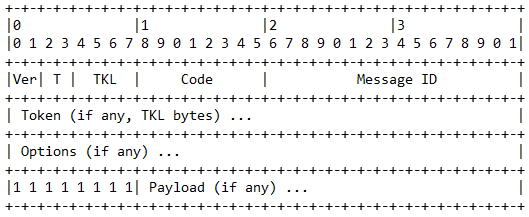
\includegraphics[width=0.8\textwidth]{MESSAGE_FORMAT}
	\caption{Formato da mensagem}
	\label{fig:message_format}
\end{figure}
%

\subsubsection{Cabeçalho}

Composto de: 
\begin{itemize}
	\item \textbf{Versão (Ver):} 2 bits do tipo  \textit{unsigned integer}. Valor 01, deve ser setado como 01, outros valores reservados. Caso receba mensagens com valor diferente, mensagem deve ser ignorada;
	\item \textbf{Tipo (T):} 2 bits do tipo  \textit{unsigned integer}, indica o tipo da mensagem, sendo: \textit{Confirmable} (0), \textit{Non-confirmable} (1), \textit{Acknowledgement} (2) ou \textit{Reset} (3);
	\item \textbf{Tamanho do \textit{Token}:} 4 bits do tipo  \textit{unsigned integer}. Indica o tamanho do campo \textit{token}, podendo ser de 0 a 8 bytes, valores de 0 a 8. Valores 9 a 15 reservados, caso a mensagem tenha algum desses valores, lidar como erro;
	\item \textbf{\textit{Code:}} 8 bits do tipo  \textit{unsigned integer}. Os 3 bits do tipo  \textit{unsigned integer} mais significantes são a classe, e outros 5 bits dão detalhes da mensagem, similar a resposta do protocolo HTTP. Veremos com detalhes no capítulos de pedidos e respostas, mas o eles são classificados conforme os 3 bits mais significativos:
	\begin{itemize}
		\item \textbf{0: } Indica pedido.
		\item \textbf{2: } Indica resposta bem sucedida.
		\item \textbf{4: } Resposta do cliente com erro.
		\item \textbf{5: } Resposta do servidor com erro.
		\item Código 0.00 indica mensagem vazia e demais códigos são reservados, outros códigos mais detalhados na imagem \ref{fig:cod_resp}. %%%%TABELA OU IMAGEM
		%%TABELA %%
	\end{itemize}
	\begin{figure}[!htb]
		\centering
		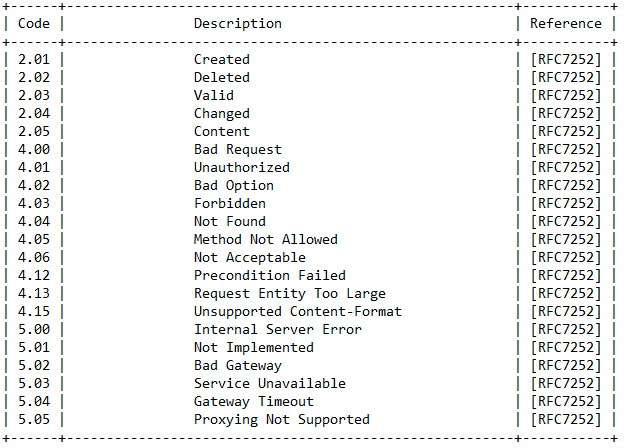
\includegraphics[width=0.8\textwidth]{CODE_RESPOSTAS}
		\caption{Códigos de resposta}
		\label{fig:cod_resp}
	\end{figure}
	\item \textit{\textbf{Message ID:}} 16 bits do tipo \textit{unsigned integer} em ordem, usado para detectar mensagens duplicadas e para combinar mensagens de ACK/\textit{Reset} com mensagens do tipo \textit{Confirmable}/\textit{Non-confirmable}.
\end{itemize}

\subsubsection {\textit{Token}}

Pode ser de tamanho entre 0 a 8 bytes, como determinado no campo TKL, é usado para relacionar pedidos e respostas.

\subsubsection {Opções}
\label{subsubsubsection{coap_option}}

O padrão CoAP define um número de opções máximas que pode ser incluído na mensagem. Cada opção deve incluir o número da opção, seguido do tamanho do valor da opção e por último o valor da opção. A imagem \ref{fig:opcoes_format} seguir demonstra como são formadas as opções. Abaixo estão suas definições:
\begin{figure}[!htb]
	\centering
	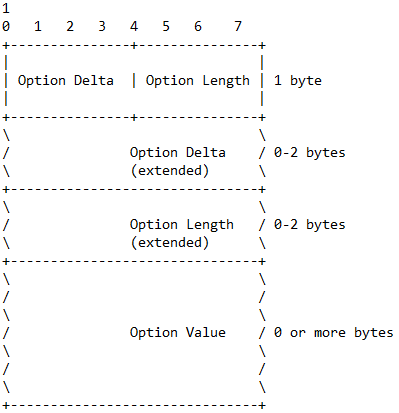
\includegraphics[width=0.8\textwidth]{OPTIONS}
	\caption{Formato Opções}
	\label{fig:opcoes_format}
\end{figure}

\begin{itemize}
	\item \textit{\textbf{Option Delta: }}4 bits do tipo \textit{unsigned integer}. Um valor entre 0 a 12 indica o valor do Delta da opção. Três valores são reservados.
	\begin{itemize}
		\item \textbf{13: }Um valor do tipo \textit{unsigned integer} de 8 bits segue o byte inicial e indica o \textit{Option Delta} menos 13.
		\item \textbf{14: }Um valor do tipo \textit{unsigned integer} de 16 bits segue o byte inicial e indica o \textit{Option Delta} menos 269.
		\item \textbf{15: }Reservado para \textit{Payload Marker}.
	\end{itemize}
	\item \textit{\textbf{Option Length: }} 4 bits do tipo \textit{unsigned integer}. Um valor entre 0 a 12  indicando o tamanho do valor da opção, em bytes. Três valores são reservados.
	\begin{itemize}
		\item \textbf{13: }Um valor do tipo \textit{unsigned integer} de 8 bits segue o byte inicial e indica o \textit{Option Length} menos 13.
		\item \textbf{14: }Um valor do tipo \textit{unsigned integer} de 16 bits segue o byte inicial e indica o \textit{Option Lenght} menos 269.
		\item \textbf{15: }Reservado para \textit{Payload Marker}.
	\end{itemize}
	\item \textit{\textbf{Option Value:}} O valor da opção não é definido diretamente, ele deve ser calculado utilizando o valor da opção e um delta. Sendo calculado da seguinte forma, o valor da opção atual é igual a soma do delta, o campo enviado na mensagem, mais o número da Opção anterior que deve ser armazenado no servidor. O valor inicial da opção anterior será zero. Além disso, o valor da opção segue os seguintes formatos:
	\begin{itemize}
		\item \textit{empty}: Uma sequência de bits de tamanho 0, indicando um valor vazio.
		\item \textit{opaque}: Uma sequência de bits cuja estrutura de dados não está definida.
		\item \textit{uint}: Um inteiro não negativo representado em ordem usando números de bytes dados. Deve ser definido e deve representar inteiros com o menor número de bytes possível.
		\item \textit{string}: Uma string codificada em UTF-8 na forma Net-Unicode \cite{rfc7252_CoAP}.	
	\end{itemize}
\end{itemize}
Possíveis valores de opção conforme tabela \ref{coap_opcoes}.
\begin{table}[!htb]
	\centering
	\caption{Opções CoAP}
	\label{coap_opcoes}
	\begin{tabular}{l|l|l}
		Number & Name           & Reference  \\ \hline
		0      & (Reserved)     & [RFC7252]  \\ \hline
		1      & If-Match       & [RFC7252]  \\ \hline
		3      & Uri-Host       & [RFC7252]  \\ \hline
		4      & ETag           & [RFC7252]  \\ \hline
		5      & If-None-Match  & [RFC7252]  \\ \hline
		7      & Uri-Port       & [RFC7252]  \\ \hline
		8      & Location-Path  & [RFC7252]  \\ \hline
		11     & Uri-Path       & [RFC7252]  \\ \hline
		12     & Content-Format & [RFC7252]  \\ \hline
		14     & Max-Age        & [RFC7252]  \\ \hline
		15     & Uri-Query      & [RFC7252]  \\ \hline
		17     & Accept         & [RFC7252]  \\ \hline
		20     & Location-Query & [RFC7252]  \\ \hline
		35     & Proxy-Uri      & [RFC7252]  \\ \hline
		39     & Proxy0Scheme   & [RFC7252]  \\ \hline
		60     & Size1          & [RFC7252]  \\ \hline
		128    & (Reserved)     & [RFC7252]  \\ \hline
		132    & (Reserved)     & [RFC7252]  \\ \hline
		136    & (Reserved)     & [RFC7252]  \\ \hline
		140    & (Reserved)     & [RFC7252] 
	\end{tabular}
\end{table}

\hfill \break
\hfill \break
\hfill \break
\hfill \break
\hfill \break
\hfill \break
\subsubsection {\textit{Payload}}

Deve ser indicado com um byte chamado \textit{Payload Marker}, de valor 0xFF, que indica o fim das opções e início do \textit{payload}. Terá o tamanho definido pelo final do pacote UDP, a partir do byte \textit{Payload Marker}. Caso não haja um \textit{Payload Marker}, o \textit{payload} deve ser lido como tamanho zero. Caso exista um \textit{Payload Marker} não seguido por um \textit{payload} de tamanho zero, tratar como erro.

\subsection{Confiabilidade}

A troca de mensagens entre nós de forma confiável é feita com o uso de mensagens Confimable. Esse tipo de mensagem sempre carrega um pedido ou uma resposta, a não ser que seja usada para \textit{Reset}, sendo uma mensagem vazia.
O servidor deve mandar um ACK em uma mensagem \textit{Confirmable} ou rejeitar a mensagem caso não possa processar, enviando uma mensagem de \textit{Reset} ou ignorando a mensagem. O ACK deve repetir o campo \textit{Message ID} da mensagem \textit{Confirmable} e carregar uma resposta ou ser vazia.  Caso ele envie o conteúdo da resposta no mesmo pacote do ACK, chamamos isso de Piggybacked response.
O cliente ou servidor enviarão a mensagem em intervalos crescentes, até receber um ACK, ou \textit{Reset}, ou ainda ficar sem tentativas de envio, como veremos a seguir.
A retransmissão é controlada através de dois parâmetros, que devem ser gerenciadas pelo dispositivo transmissor, para cada mensagem \textit{Confirmable}, um \textit{timeout} e um contador de retransmissões. Para cada retransmissão, o \textit{timeout} é dobrado, iniciando de um valor randômico entre ACK\_TIMEOUT e (ACK\_TIMEOUT x ACK\_RANDOM\_FACTOR), conforme tabela abaixo. O transmissor ainda pode desistir da mensagem caso a mensagem perca o propósito ou receba outros erros a serem tratados.
Mensagens não confiáveis podem ser utilizadas também, sendo útil em casos de uma mensagem que é transmitida regularmente e de mesmo conteúdo, utilizando o modo \textit{\textit{Non-confirmable}}.
Para manter o tráfego controlado, o padrão CoAP também limita o número máximo de iterações simultâneas para um valor configurável, NSTART.


\subsection{Correlação da mensagem e mensagens duplicadas}

As mensagens são relacionadas através do campo \textit{Message ID} com uma informação adicional do endpoint. O \textit{Message ID} é um valor de 16 bits do tipo \textit{unsigned integer}, gerado pelo transmissor. Esse \textit{Message ID} deve ser copiado na resposta em uma mensagem do tipo ACK ou \textit{Reset} pelo receptor. Além disso, o \textit{Message ID} não deve ser reutilizado, com o mesmo endpoint, dentro do tempo EXCHANGE\_LIFETIME, figura \ref{coap_parametro_deriv}.
O receptor pode coletar mais de uma mensagem \textit{Confirmable} com mesmo conteúdo, pode ser descoberto comparando a \textit{Message ID} e o nó fonte, múltiplas vezes dentro do EXCHANGE\_LIFETIME, ele deve enviar mensagens de ACK ou \textit{Reset} para todas as mensagens duplicadas recebidas, porém, só deve processar a mensagem uma vez.


\subsection{Tamanho da mensagem}

O padrão CoAP se beneficia de mensagens pequenas, facilitando tanto na criação da mensagem pelo embarcado, quanto para a rede, mas ele não estabelece um tamanho mínimo, apenas um tamanho máximo, porém uma mensagem maior que um pacote IP resulta em fragmentação da mensagem, portanto o padrão sugere que a mensagem seja menor que um pacote IP.

\subsection{Parâmetros de transmissão}

Os valores padrões utilizados para retransmissão seguem os valores da tabela \ref{coap_parametro_default}.

\begin{table}[!htb]
	\centering
	\caption{Parâmetros padrões CoAP}
	\label{coap_parametro_default}
	\begin{tabular}{l|l}
		\hline
		name                & default vale  \\ \hline
		ACK\_TIMEOUT        & 2 seconds     \\ \hline
		ACK\_RANDOM\_FACTOR & 1.5           \\ \hline
		MAX\_RETRANSMIT     & 4             \\ \hline
		NSTART              & 1             \\ \hline
		DEFAULT\_LEISURE    & 5 seconds     \\ \hline
		PROBING\_RATE       & 1 byte/second \\ \hline
	\end{tabular}
\end{table}

Ainda podemos calcular outros valores, derivados dos primeiros, que são utilizados no padrão, conforme podemos ver na tabela \ref{coap_parametro_deriv}. Para mais detalhes, consultar a RFC7252 \cite{rfc7252_CoAP}.

\begin{table}[!htb]
	\centering
	\footnotesize\setlength{\tabcolsep}{25pt}
	\caption{Parâmetros derivados CoAP}
	\label{coap_parametro_deriv}
	\begin{tabular}{l|r}
		\hline
		name                & \multicolumn{1}{l}{default value} \\ \hline
		MAX\_TRANSMIT\_SPAN & 45 s                               \\ \hline
		MAX\_TRANSMIT\_WAIT & 93 s                               \\ \hline
		MAX\_LATENCY        & 100 s                              \\ \hline
		PROCESSING\_DELAY   & 2s                                 \\ \hline
		MAX\_RTT            & 202 s                              \\ \hline
		EXCHANGE\_LIFETIME  & 247 s                              \\ \hline
		NON\_LIFETIME       & 145 s                              \\ \hline
	\end{tabular}
\end{table}


\subsection{Pedidos e respostas}


Um pedido CoAP consiste em, um método que será aplicado, o identificador do recurso, o \textit{payload}, um \textit{Internet media type}, se presente e um \textit{metadata} opcional sobre o pedido. É identificado no campo \textit{code} do \textit{header}. Ele pode ser do tipo GET, POST, PUT e DELETE, seguindo a denominação do padrão HTTP para facilitar o entendimento deste novo padrão, conforme veremos a seguir na tabela \ref{coap_code_method}. Eles são \textit{idempotents}, ou seja, pode se invocar múltiplas vezes com mesmo efeito, com exceção do POST porque a sua função é determinada dependendo do recurso alvo.
A resposta é identificada da mesma forma, no campo \textit{code} do \textit{header}, tabela \ref{coap_resposta_code}, e indica o resultado da tentativa de entender o pedido.
As mensagens de pedido e resposta são relacionadas através do \textit{token}, ao invés do \textit{Message ID} como é feito com mensagens \textit{Confirmable} ou \textit{Non-confirmable} e \textit{Acknowledgement} ou \textit{Reset}.

\begin{table}[!htb]
	\centering
	\caption{Métodos CoAP pedido (\textit{code} \textit{header})}
	\label{coap_code_method}
	\begin{tabular}{l|l|l}
		\hline
		Code & Name    & Reference     \\ \hline
		0.01 & GET     & {[}RFC7252{]} \\ \hline
		0.02 & POST    & {[}RFC7252{]} \\ \hline
		0.03 & PUT     & {[}RFC7252{]} \\ \hline
		0.04 & DELETE  & {[}RFC7252{]} \\ \hline
	\end{tabular}
\end{table}

\begin{table}[!htb]
	\centering
	\footnotesize\setlength{\tabcolsep}{25pt}
	\caption{Código de respostas (\textit{code} \textit{header})}
	\label{coap_resposta_code}
	\begin{tabular}{l|l|l}
		\hline
		Code & Description                & Reference     \\ \hline
		2.01 & Created                    & {[}RFC7252{]} \\ \hline
		2.02 & Deleted                    & {[}RFC7252{]} \\ \hline
		2.03 & Valid                      & {[}RFC7252{]} \\ \hline
		2.04 & Changed                    & {[}RFC7252{]} \\ \hline
		2.05 & Content                    & {[}RFC7252{]} \\ \hline
		4.00 & Bad Request                & {[}RFC7252{]} \\ \hline
		4.01 & Unauthorized               & {[}RFC7252{]} \\ \hline
		4.02 & Bad Option                 & {[}RFC7252{]} \\ \hline
		4.03 & Forbidden                  & {[}RFC7252{]} \\ \hline
		4.04 & Not Found                  & {[}RFC7252{]} \\ \hline
		4.05 & Method Not Allowed         & {[}RFC7252{]} \\ \hline
		4.06 & Not Acceptable             & {[}RFC7252{]} \\ \hline
		4.12 & Precondition Failed        & {[}RFC7252{]} \\ \hline
		4.13 & Request Entity Too Large   & {[}RFC7252{]} \\ \hline
		4.15 & Unsopported Content-Format & {[}RFC7252{]} \\ \hline
		5.00 & Internal Server Error      & {[}RFC7252{]} \\ \hline
		5.01 & Not Implemented            & {[}RFC7252{]} \\ \hline
		5.02 & Bad Gateway                & {[}RFC7252{]} \\ \hline
		5.03 & Service Unavailable        & {[}RFC7252{]} \\ \hline
		5.04 & Gateway Timeout            & {[}RFC7252{]} \\ \hline
		5.05 & Proxying Not Supported     & {[}RFC7252{]} \\ \hline
	\end{tabular}
\end{table}


\subsection{Métodos}

Os métodos aceitos serão citados abaixo, caso haja um pedido com método não reconhecido ou não suportado, deve ser gerada uma \textit{Piggybacked response} \ref{subsection:msg_piggybacked} do tipo 4.05, método não permitido.

\subsubsection {GET}

Solicita a informação sobre o recurso identificado na URI.  Tipo de mensagem \textit{Non-Confirmable}.

\subsubsection {POST}
\label{subsubsection:post}
A função do método é determinada pelo servidor de origem e depende do recurso alvo. Usualmente resulta na criação de um novo recurso ou atualização do recurso alvo já existente. Tipo de mensagem \textit{Confirmable}.

\subsubsection {PUT}

O método PUT solicita que o recurso identificado na URI seja criado ou atualizado. Tipo de mensagem \textit{Non-Confirmable}.

\subsubsection {DELETE}

Define que o recurso identificado pela URI seja excluído.

\section{ESP8266}

É um módulo, de tamanho reduzido e baixo custo. Além de, nas suas versões mais atuais, ter a facilidade de comunicação micro-USB para implementação de código. Ele pode também ser utilizado de forma integrada a outro sistema embarcado utilizando a comunicação UART, para implementar a função de comunicação com a internet.


Ele existe em diversas versões, mas todas com praticamente o mesmo funcionamento. Sua CPU é baseada em um IP Xtensa, da Cadence, levemente modificado pela empresa fabricante Espressif.
Alguns de seus recursos de hardware são:

\begin{itemize}
	\item Conectores GPIO, barramentos I2C, SPI, UART, entrada ADC, saída PWM e sensor interno de temperatura;
	\item CPU que opera em 80MHz, com possibilidade de operar em 160MHz;
	\item Arquitetura RISC de 32 bits;
	\item 32KBytes de RAM para instruções;
	\item 96KBytes de RAM para dados;
	\item 64KBytes de ROM para boot;
	\item O núcleo é baseado no IP Diamand Standard LX3 da Tensilica;
	\item Fabricado pela Espressif;
	\item VCC de 3,3V para operar.
\end{itemize}

E algumas características de funcionamento são:
\begin{itemize}	
	\item Engine integrada para criptografias WEP, TKIP, AES e WPA;
	\item Suporte aos protocolos 802.11 b/g/n;
	\item Wi-Fi Direct (P2P), soft-AP;
	
	\item Pilha de protocolo TCP/IP integrada com suporte a IPv4;
	\item Wi-Fi em frequência de 2.4GHz com suporte a WPA e WPA2;
	\item Potência de saída em +20dBm no modo 802.11b;
	
	\item Conversor ADC integrado com resolução de 10 bits;
	\item Suporte a uma variedade de antenas;
	\item Energia de consumo em modo sleep menor que 10uA;
	
	\item Tempo para sair de sleep e transmitir pacotes menor que 2ms;
	\item Potência de standby menor que 1.0mW;
	\item Pode operar em faixa de temperaturas de -40ºC a 125ºC.
	
\end{itemize}

A empresa desenvolvedora Espressif \cite{espressif_ref} disponibiliza um repositório no GitHub para facilitar o desenvolvimento para este microcontrolador, com alguns exemplos já desenvolvidos \cite{esp8266_site}.
\chapter{Desenvolvimento}

Algumas ferramentas foram fundamentais para o desenvolvimento deste projeto, a seguir descreverei as principais ferramentas utilizadas.

\section{Ferramentas utilizadas}

\subsection{VMWare Workstation Player}

Utilizado para executar máquinas virtuais \cite{vmware_player_ref}, no meu caso, com distribuições linux, Ubuntu\cite{ubuntu_ref} e Linux Mint\cite{linux_mint_ref}, para desenvolvimento do cliente e servidor C. Utilizei essa plataforma pela facilidade e confiabilidade necessárias para o desenvolvimento. O linux possui bibliotecas nativas que usei para compilação e execução do cliente e servidor.

\subsection {Eclipse}

Utilizado para escrita \cite{eclipse_ref}, em conjunto com o guia para windows \cite{devkit_windows_ref}, no embarcado. Com este tutorial, foi possível fazer o \textit{flash} de alguns projetos já existentes para teste do hardware em si.

\subsection{Putty}

Utilizado para ler as respostas do sistema embarcado, recebendo através da porta USB a resposta da execução do mesmo \cite{putty_ref}.

\subsection {SoAP UI}

Utilizado para testar a comunicação com o WebServer da empresa\cite{soap_ui_ref}.


\section{Projeto}

A partir do desenvolvimento de uma aplicação, que pode ser embarcada em um hardware modesto e utilizada com conexões precárias, em conjunto de diversos tipos de sensores visa-se atender este mercado de monitoramento e controle de ambientes. Assim, tratar-se-á, neste capítulo, sobre o desenvolvimento do projeto de cliente e servidor CoAP, em que é possível visualizar a implementação exposta no diagrama abaixo.

\begin{figure}[!htb]
	\centering
	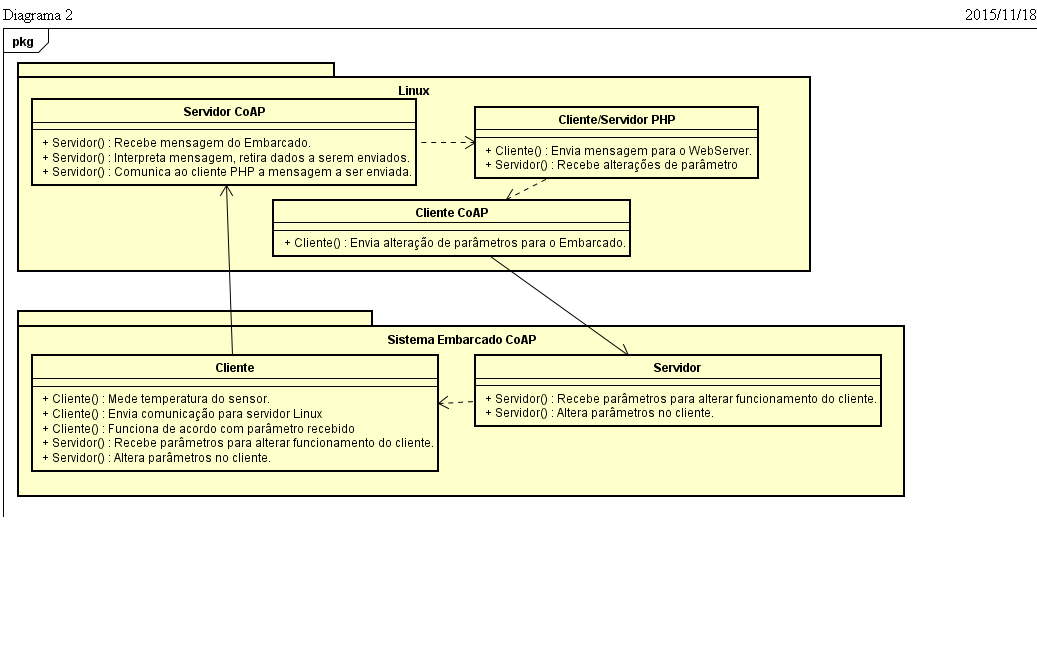
\includegraphics[width=1.0\textwidth]{../Diagrama_sem_webserver.png}
	\caption{Diagrama 1}
	\label{fig:Diagrama_lin_emb}
\end{figure}


Ainda que demonstrados cliente e servidor juntos, este projeto foi pensado e desenvolvido para ser utilizado de forma separada também. A implementação de ambos os elementos será descrita individualmente, e, por fim, será descrito o funcionamento delas em conjunto. Em mais detalhes, todo o código pode ser visto em \cite{cliente_servidor_coap}.

\section{Cliente CoAP}
O cliente foi desenvolvido em C, visando a aumentar a possibilidade de implantação em embarcados de baixo custo e melhoria de performance. A mensagem será transportada pelo protocolo UDP, utilizando o protocolo de aplicação CoAP. O funcionamento será dividido e descrito nas próximas seções para melhor entendimento.


\subsection{Conexão}
Como visto, utilizar-se-á o protocolo UDP para transporte, então, a conexão será feita, como demonstrada abaixo:

\begin{figure}[!htb]
	\begin{lstlisting}
	//CONEXAO
	int fd;
	
	struct sockaddr_in servaddr;
	fd = socket(AF_INET,SOCK_DGRAM,0);
	bzero(&servaddr,sizeof(servaddr));
	servaddr.sin_family = AF_INET;
	servaddr.sin_addr.s_addr = inet_addr("192.168.1.20");
	servaddr.sin_port = htons(7891);
	bind(fd,(struct sockaddr *)&servaddr, sizeof(servaddr));
	\end{lstlisting}
	\caption{Conexão do cliente, via porta 7891}
	\label{code:conexao_cliente}
\end{figure}

Ao ligar o socket à porta e ao endereço do servidor, via UDP, o envio da mensagem é feito da seguinte forma

\begin{figure}[!htb]
	\begin{lstlisting}
	if (rand()%100<PORCENTAGEM)
	{
	printf("\n\nEnviando\n\n");
	sendto(fd, buf_out, rsplen, 0, (struct sockaddr *) &cliaddr, sizeof(cliaddr));
	}
	else
	{
	printf("\n\nNão enviando, simulando erro de comunicação\n\n");
	}    
	\end{lstlisting}
	\caption{Simulação de erro de conexão}
	\label{code:simulacao_erro_conexao}
\end{figure}

Foi utilizada a função \texttt{if(rand()\%100<PORCENTAGEM)} para simular a perda de pacotes em conexões limitadas.


\subsection{Criação do pacote}

Foi usada a função \texttt{cria\_pkt }, e essa, por sua vez, chama a função  \texttt{monta\_header\_token} \ref{code:monta_header_token}, para criação do \textit{header} e \textit{token} do pacote, que são pré-definidos, no caso de o \textit{token} utilizado ser gerado pelo programa e não pelo usuário. Um pequeno trecho dela é visto na figura logo abaixo.

Foram empregadas também as funções \texttt{srand, rand()} para gerar aleatoriamente valores para o \textit{id} e para o \textit{token}, gerado de forma similar à utilizada para criar o \textit{id}, porém não foi transposta para o trecho abaixo.

\begin{figure}[!htb]
	\begin{lstlisting}
	void monta_header_token (coap_packet_t *pkt, uint8_t *token)
	{
		pkt->hdr.ver = 	 0x01; // versão 01;
		pkt->hdr.t = 	 0x00; // code 0 (confirmable);
		pkt->hdr.code =  0x02; //request -> 0000 0010 -> POST, 0000 0011 -> PUT
		srand(time(NULL));
		short int var_aux = rand()%254;
		pkt->hdr.id [0] = var_aux;
		short int var_aux = rand()%254;
		pkt->hdr.id [1] = var_aux;
		...
		pkt->tok.p = token;
		pkt->tok.len = strlen(token);
		pkt->hdr.tkl = pkt->tok.len;
	}
	\end{lstlisting}
	\caption{Pequeno trecho da função \texttt{monta\_header\_token}}
	\label{code:monta_header_token}
\end{figure} 

\subsection{Parâmetros}
\label{subsection:parametros}

Inicialmente, foi pensado em receber os parâmetros via linha de comando, passando-os como argumentos para a função, porém, além de dificultar os testes, posteriores à criação do cliente, pensou-se em fazer do cliente uma função do servidor. Para isso, uma mensagem padrão foi criada, com \textit{options} definidas e necessitando alterar apenas o \textit{payload}, com \textit{token} gerado de forma aleatória.
Como a função de identificação e verificação de parâmetros já havia sido feita para receber os parâmetros via linha de comando, apenas foi necessária uma adaptação da mensagem, para se encaixar nos moldes utilizados pela função padrão de recebimento de parâmetros; assim, a função seguinte de identificação não faz distinção entre o método empregado para envio de parâmetros utilizado.
A função utilizada para este fim, de alterar a mensagem pré-pronta deixando-a nos moldes da versão anterior, foi a \texttt{separa\_string}.

\subsection{Verificação e interpretação dos argumentos}

Aqui será utilizada parte da função \texttt{identifica\_arg} \ref{code:identifica_arg} para explicar como foi feita a identificação dos argumentos.

\begin{figure}[!htb]
	\begin{lstlisting}
	void identifica_arg (coap_packet_t *pkt, int argc, char **argv, char *buf_aux_opt_c, short int *buf_aux_opt_n)
	{
		...
		else if(strcmp(argv[j], "-op") == 0)
		{
			if (j+3 > argc) //caso não tenha os campos necessários
			{
				lida_erro_id(erro_argumento_num_option_invalido, argc, argv);
			}
			else if(veri_option (argv[j+1], argv[j+2]))
			{
				lida_erro_id(erro_argumento_num_option_invalido, argc, argv);
			}
			else
			{
				add_option(pkt, cont_aux, &buf_aux_opt_n[cont_op-1], argv[j+2], cont_op, &option_delta);
				j+=3;
			}
		}
		...
	}
	\end{lstlisting}
	\caption{Trecho da função \texttt{identifica\_arg} demonstrando a ação dela}
	\label{code:identifica_arg}
\end{figure}
\hfill \break
\hfill \break
\hfill \break
\hfill \break
\hfill \break
\hfill \break
\hfill \break
\hfill \break
\hfill \break
\hfill \break
\hfill \break

Como é possível ver na figura \ref{code:identifica_arg}, é feita uma verificação dos parâmetros, para averiguar se são argumentos válidos, com a função \texttt{veri\_option} e, caso sejam, sãoo adicionados ao pacote criado. A seguir, serão descritas, com mais detalhes, as funções \texttt{add\_token}, \texttt{add\_option} e \texttt{add\_payload}. 

\subsubsection{Funções de adicionar \textit{payload}, \textit{option}, \textit{token}}

Estas três funções \texttt{add\_token}, \texttt{add\_option} e \texttt{add\_payload} são utilizadas para adicionar o conteúdo da mensagem ao pacote, respectivamente, inserindo \textit{token}, \textit{options} e \textit{payload}. Elas têm funcionamento similar, copiando o conteúdo do buffer para o pacote e respeitando as especificações de tamanho da tabela \ref{table:valores_token_option_payload}.

\begin{table}[!htb]
	\centering
	\caption{Definições de tamanho para \textit{token}, \textit{option}, \textit{payload}}
	\label{table:valores_token_option_payload}
	\begin{tabular}{l|l}
		Tamanho máximo  & Valor em bytes \\ \hline
		Token tamanho   & 9              \\ \hline
		Option conteúdo & 24             \\ \hline
		Payload         & 64             \\ \hline
		Delta valor     & 64            
	\end{tabular}
\end{table}

\subsection{Monta pacote}

A mensagem é montada no pacote (\texttt{\&pkt}) e enviada através do buffer de saída (\texttt{buf\_out}). Essa tarefa é feita pela função \texttt{monta\_pkt}.
\begin{figure}[!htb]
	\begin{lstlisting}
	void monta_pkt (coap_packet_t *pkt, uint8_t *buf)
	{
		uint16_t running_delta = 0;
		char tempo[100];
		tempo_agora(tempo);
		...
		//Montando header
		buf[0] = (pkt->hdr.ver & 0x03) << 6;
		buf[0] |= (pkt->hdr.t & 0x03) << 4;
		buf[0] |= (pkt->hdr.tkl & 0xFF);
		buf[1] = pkt->hdr.code;
		buf[2] = pkt->hdr.id[0];
		buf[3] = pkt->hdr.id[1];
		p = buf+4;
		...
		//Montando token
		memcpy(p, pkt->tok.p, pkt->hdr.tkl);
		p = p+pkt->hdr.tkl;
		...
		//Montando options
		short int aux = (short int)pkt->numopts;
		for (i=0; i<aux; i++)
		{
			...
			memcpy(p, pkt->opts[i].buf.p, pkt->opts[i].buf.len);
			p = p + pkt->opts[i].buf.len;
		}
		...
		//Montando payload
		*p++ = 0xFF;
		memcpy(p, pkt->payload.p, pkt->payload.len);
		p = p+pkt->payload.len;
		
		//Adicionando tempo
		memcpy(p, tempo, (int)strlen(tempo));
		p=p+(int)strlen(tempo);
	}
	\end{lstlisting}
	\caption{Trecho da função \texttt{monta\_pkt} demonstrando a ação dela}
	\label{code:montar_pkt}
\end{figure}

É a função \texttt{monta\_pkt} também que faz o controle do parâmetro \texttt{running\_delta}, explicado na seção de opções do CoAP \ref{subsubsubsection{coap_option}}.

Ainda nela, é utilizada a função \texttt{tempo\_agora}, com objetivo de calcular o tempo no instante de execução. Através desse parâmetro, será calculado o desempenho do cliente. Abaixo será descrito, de forma simplificada, o funcionamento dessa função.

\verb||

\subsection{PUT}

A partir deste momento, a mensagem já foi montada, copiada para buffer e enviada, então, o cliente já está pronto e executando sua tarefa. 

Em caso de o tipo de mensagem ser PUT \ref{subsubsection:post}, o cliente já foi finalizado, necessitando apenas da função \texttt{separa\_string}, como discutido no tópico anterior Parâmetros \ref{subsection:parametros}, caso queira ser utilizada uma \textit{string} pré-definida para envio. O controle de tempo também é feito após o envio da mensagem e enviado para o arquivo de log.

\subsection{POST}

Para mensagens do tipo POST \ref{subsubsection:post}, foram utilizadas mais algumas funções adicionais: a  função de armazenar mensagem em buffer, \texttt{buffer\_msg} e a função para lidar com mensagem recebida \texttt{lida\_msg\_recebida}.

O tipo POST ainda realizará cinco tentativas de envio da mensagem, em caso de não recebimento do ACK.

\subsubsection{Separação de palavras}
A função \texttt{separa\_string} \ref{code:separa_string} tem objetivo de separar todos os parâmetros de uma \textit{string} única. Foi utilizado a variável \texttt{string\_sep}, que é alocada dinamicamente, conforme a \textit{string} que está sendo passada.

\begin{figure}[!htb]
	\begin{lstlisting}
	void separa_string (char **string_sep, char *buf, short int n_str, short int len)
	{
		for (i=0; i<len; i++)
		{
			if (buf[i] == ' ')
			{			
				string_sep[count_w][j] = '\0';
				count_w++;
				j=0;
			}
			else
			{
				string_sep[count_w][j] = buf[i];
				j++;
			}
		}
	}
	\end{lstlisting}
	\caption{Pequeno trecho da função \texttt{separa\_string}}
	\label{code:separa_string}
\end{figure}


\subsubsection{Buffer}

Esta função foi pensada para controlar o buffer, buscando uma posição vazia para armazenar a mensagem e escrevendo nesta posição do buffer. Ela também faz controle da capacidade do buffer, retornando uma mensagem de erro em caso de o buffer já estar cheio. Aqui poderia ser implementada outra forma de lidar com esse erro, a partir da reescritura sobre uma posição ocupada ou do descarte das mensagens para limpar o buffer após certo tempo. Um pequeno trecho da função é vista na figura \ref{code:buffer_msg}.

\begin{figure}[!htb]
	\begin{lstlisting}
	void buffer_msg (char *buf_out, char *buf_out_p, short int *cont_msg, short int *pos, char buf_str[][512])
	{
		int k, m, ult_esc = -1;
		if(*cont_msg > 7)
		{
			lida_erro_buffer (erro_buffer_cheio);
		}
		...
		else
		{
			k=1;
			while(k==1)
			{
				if(ult_esc == 7)
				{
					ult_esc = -1;
				}
				if(pos[ult_esc+k]==0)
				{
					...
					ult_esc++;
					*cont_msg = *cont_msg + 1;;
					pos[ult_esc] = 1;
					memcpy(buf_str[ult_esc], buf_out, 512);
					...
					break;
				}
			ult_esc++;
		}
	}
	\end{lstlisting}
	\caption{Pequeno trecho da função \texttt{buffer\_msg}}
	\label{code:buffer_msg}
\end{figure}

\subsubsection{Espera e reenvio da mensagem}

No caso de um POST, após a mensagem ser enviada, tem-se a espera pela resposta. Essa espera foi feita respeitando um parâmetro, o \texttt{NUM\_TIMEOUT}, que foi setado antes da execução, e é o limite máximo de tentativas que o cliente fará para envio da mensagem. É utilizada também a função \texttt{setsockopt} para fazer a espera pela mensagem por um período de tempo determinado pelos parâmetros \texttt{ACK\_WAIT\_TIMEOUT\_SEC} e \texttt{ACK\_WAIT\_TIMEOUT\_USEC}, respectivamente, a quantidade de segundos e micro-segundos em que o cliente esperará.

Então, recebida a mensagem, foi utilizada a função \texttt{lida\_msg\_recebida} para lidar com a mensagem do servidor que chega ao cliente, que seria a mensagem de ACK. E caso ela não seja recebida, a mensagem enviada deve ser reenviada. Conforme a figura \ref{code:envio_post}. 

\begin{figure}[!htb]
	\begin{lstlisting}
	while (num_timeouts < NUM_TIMEOUT)
	{
		if (setsockopt(fd, SOL_SOCKET, SO_RCVTIMEO,&tv,sizeof(tv)) < 0) 
		{
			perror("Error");
		}		
		else if (recvfrom(fd, buf_in, rsplen, 0, (struct sockaddr *)&cliaddr, &szcliaddr) >= 0)
		{
		
			if (1 == lida_msg_recebida (buf_in, buf_str, &cont_msg, pos, &time_post, &time_start, pFile))
			{
				num_timeouts = NUM_TIMEOUT;
			}			   		
		}
		else
		{
			printf("Entrando no msg não recebida, reenviando\n");
			if (rand()%100<PORCENTAGEM)
			{
				printf("\n\nEnviando\n\n");
				sendto(fd, buf_out, rsplen, 0, (struct sockaddr *) &cliaddr, sizeof(cliaddr));
			}
			else
			{
				printf("\n\nNot sending, simulando erro de comunicação\n\n");
			}
		}
	}
	\end{lstlisting}
	\caption{Pequeno trecho do cliente método POST}
	\label{code:envio_post}
\end{figure}

\subsubsection{Lida com mensagem recebida}

Essa função, \texttt{lida\_msg\_recebida} \ref{code:lida_msg_recebida} foi utilizada para comparar a mensagem recebida com a armazenada e para confirmar se é o ACK esperado. Caso a mensagem seja ACK, deve retornar 1, caso contrário, retornará 0.

Ela faz isso, comparando inicialmente o \textit{header} das duas mensagens, à armazenada e à recebida, e, entãom passa a comparar o restante da mensagem, até o final das \textit{options}.

\begin{figure}[!htb]
	\begin{lstlisting}
	int lida_msg_recebida (char *buf_in, char buf_str[][512], short int *cont_msg, short int *pos, struct timespec *time_post, struct timespec *time_start, FILE *pFile)
	{
		for (i=0; i<8; i++)
		{
			if (pos[i] == 1)
			{
				if (((buf_in[0] & (0xF0)) == 0x60) && ((buf_in[0] & 0X0F) == (buf_str[i][0] & 0x0F)) && ((buf_in[1] & 0xFF )== 0x44))
				{
					int cont = 0;
					for (j=0; j<(buf_in[0] & 0x0F); j++)
					{
						if(buf_in[2+j] == buf_str[i][2+j])
						{
							cont++;
						}
					}
					if (cont == (buf_in[0] & 0x0F))
					{
						pos[i] = 0;
						*cont_msg = *cont_msg - 1;
						memset(buf_str[i], 0x00, 512);
						return 1;
					}
				}
				else
				{
					return 0;
				}
			}
		}
	}
	\end{lstlisting}
	\caption{Pequeno trecho da função \texttt{lida\_msg\_recebida}}
\label{code:lida_msg_recebida}
\end{figure}

\hfill \break
\hfill \break
\hfill \break
\hfill \break
\hfill \break
\hfill \break
\hfill \break
\hfill \break
\hfill \break

Algumas funções adicionais também foram utilizadas, descritas de forma resumida.
As funções de \texttt{printf}, como, \texttt{printf\_header} ou \texttt{printf\_buffer}, têm função de imprimir o argumento que lhes é passado: são todas funções do tipo void que não fazem modificações no dado em si.
A função \texttt{tempo\_agora} recebe uma \textit{string}, e atualiza essa \textit{string} com o tempo no instante em que a função é chamada; ela é utilizada para adicionar o tempo à mensagem que será enviada.
A função \texttt{get\_time} recebe uma estrutura de tempo e a atualiza com o tempo no instante em que é chamada, sendo utilizada para calcular o tempo de execução do programa que foi salvo nos logs.
A função \texttt{calc\_time\_sub} foi utilizada para calcular a diferença de tempo, que é dada em segundos, desde um determinado tempo até o atual.
A função \texttt{corrige\_len} foi utilizada para corrigir o tamanho da mensagem: como a mensagem do servidor continha muitas sequências de 0, o cliente estava interpretando como se não fizesse parte da mensagem; essa função corrige o tamanho do buffer interpretado.
As funções de verificação, como \texttt{veri\_token}, fazem uma validação dos caracteres recebidos. Por exemplo, um campo de número de opção deve conter apenas números, um campo de nome da opção, pode conter números e letras, e assim por diante.
As funções de lidar com erros, por exemplo, \texttt{lida\_erro\_id}, foram separadas por função que atuam, ou seja, a do exemplo lida com erros na função \texttt{identifica\_arg}, gerando um código de erro que é definido antes da compilação, no código fonte do cliente.FAZER TABELA DE ERROS%

E assim, o cliente foi finalizado e ficou apto a enviar mensagens do tipo POST e PUT. O tipo de mensagem deve ser selecionado antes da compilação, alterando o parâmetro definido POST e PUT no início do código do cliente.

\section{Servidor}

O servidor foi planejado inicialmente para testar o cliente, e, após o desenvolvimento e a alteração do projeto, pensou-se em adicionar ele também ao sistema embarcado, para garantir certa flexibilidade do cliente. Já que, com o servidor embarcado, é possível fazer pequenas alterações no funcionamento do cliente, sem necessidade de refazer o \textit{flash} no embarcado.

O servidor, diferente do cliente, não foi feito do zero. Foi realizada algumas alterações no projeto \textit{microcoap} \cite{microcoap}. As modificações serão descritas a seguir, divididas por arquivo código alterado, o código completo se encontra na \cite{microcoap}. 

\subsection{Alterações na função \textit{main}}

As alterações na \textit{main} foram feitas para comportar o cliente como função do servidor. Essa tarefa foi feita utilizando a biblioteca \textit{pthreads}, podendo ser facilmente alterada para a função \textit{fork} caso necessário. Uma \textit{thread} ficará responsável pelo servidor, e outra \textit{thread} é encarregada do cliente. A função \texttt{rand} também foi utilizada no servidor, de maneira similar a do cliente, para, através do número aleatório gerado, enviar ou não a mensagem, simulando assim erro de pacotes. Nas figuras \ref{code:thread_serv_main_posix.c} e \ref{code:main_main_posic.c} é possível verificar alguns trechos da função \texttt{main\_posix.c}.

\begin{figure}[!htb]
	\begin{lstlisting}
	void *thr_func_serv_recv (void *arg)
	{
		fd_client = socket(AF_INET,SOCK_DGRAM,0);
		servaddr.sin_family = AF_INET;
		servaddr.sin_addr.s_addr = inet_addr("192.168.252.128");
		servaddr.sin_port = htons(PORT_CLI);
		while(1)
		{
			coap_packet_t pkt;
			n = recvfrom(fd_client, buf, sizeof(buf), 0, (struct sockaddr *)&servaddr, &len);
			...
			if (0 != (rc = coap_parse(&pkt, buf, n)))
				printf("Bad packet rc=%d\n", rc);
			...
			else
			{			
				coap_packet_t rsppkt;
				coap_handle_req(&scratch_buf, &pkt, &rsppkt);
				if (0 != (rc = coap_build(buf, &rsplen, &rsppkt)))
					printf("coap_build failed rc=%d\n", rc);
				else
				{
					
					if (rand()%100<PORCENTAGEM)
					{
						printf("\n\nSending\n\n");
						sendto(fd_client, buf, rsplen, 0, (struct sockaddr *)&servaddr, sizeof(servaddr));
					}
				}
			}
		}
	}
	\end{lstlisting}
	\caption{Pequeno trecho da \textit{thread} servidor da função \texttt{main\_posix.c}}
	\label{code:thread_serv_main_posix.c}
\end{figure}


\begin{figure}[!htb]
	\begin{lstlisting}
	int main(int argc, char **argv)
	{
		endpoint_setup();
		call_cli.tv_sec = get_var_time();
		call_cli.tv_nsec = 0;
		if ((rc = pthread_create(&thr[0], NULL, thr_func_cli, &call_cli)))
		{
			fprintf(stderr, "error: pthread_create, rc: %d\n", rc);
			return EXIT_FAILURE;
		}
		if ((rc = pthread_create(&thr[1], NULL, thr_func_serv_recv, &call_cli)))
		{
			fprintf(stderr, "error: pthread_create, rc: %d\n", rc);
			return EXIT_FAILURE;
		}
	}
	\end{lstlisting}
	\caption{Pequeno trecho da função \textit{main} da \texttt{main\_posix.c}}
	\label{code:main_main_posic.c}
\end{figure}

\hfill \break
\hfill \break
\hfill \break
\hfill \break
\hfill \break
\hfill \break

\subsection{Alterações na função \textit{endpoints}}

As principais alterações aqui foram a criação de novos métodos, que seriam utilizados para armazenar dados no servidor.

O método POST de temperatura (\texttt{temperature}) foi utilizado para armazenar a temperatura recebida, em um arquivo de log, e enviar de volta como resposta à temperatura armazenada. Já o método GET de temperatura apenas envia a última temperatura salva no servidor.

O método POST de tempo (\texttt{time}) foi utilizado para armazenar o último tempo enviado, que ditará a frequência de operação do cliente, ou seja, de quanto em quanto tempo a função \texttt{main\_posix} chamará o cliente.

A implementação dessas funções pode ser vista nos anexos.

Algumas funções adicionais foram utilizadas: como a função \texttt{set\_var\_time} para a \texttt{main\_posix} fazer alteração do tempo, quando receber um pedido de outro cliente; a função \texttt{get\_var\_time}, utilizada pelo próprio sistema, para chamar o cliente de acordo com esse tempo; a função \texttt{create\_var\_time}, utilizada para a criação inicial do tempo, setado por padrão no início do código fonte da função \texttt{endpoints.c}. E a própria função \texttt{endpoints\_setup}, que chama a função \texttt{create\_var\_time} para iniciar a função \texttt{endpoints}. Essas funções podem ser vistas na figura \ref{code:endpoints.c}.

\begin{figure}[!htb]
	\begin{lstlisting}
	void endpoint_setup(void)
	{
		build_rsp();
		variable = create_var_time ();
	}
	...	
	// Variável de tempo (usar no main-posix)
	void set_var_time (short int tempo)
	{
		variable.tempo = tempo;
	}
	short int get_var_time ()
	{
		return variable.tempo;
	}
	
	var_cli create_var_time ()
	{
		var_cli variable;
		variable.tempo = 5; //Segundos, para testes
		return variable;
	}
	\end{lstlisting}
	\caption{Pequeno trecho da função \texttt{endpoints.c}}
	\label{code:endpoints.c}
\end{figure}

\chapter{Resultados}

Os testes foram feitos para comparar a taxa de entrega de pacotes, ao variar o método de envio utilizado, POST ou PUT, e a porcentagem de envio, que simula a perda de pacotes, que oscila entre 10 de 100\%.
Objetivou-se, para o teste, a simulação da perda de pacotes, já que o foco do projeto é aplicar o código em embarcados com conexão sem fio.
Todos os testes foram feitos em dois computadores, rodando o sistema operacional Linux, na distribuição Linux Mint, que visa a simular um servidor para receber os dados e o cliente embarcado que faz o envio da mensagem.

\section{PUT}

A figura \ref{fig:put_tempo_envio} mostra o primeiro teste, para comparação posterior, do tempo de envio de mensagens do tipo PUT.

\begin{figure}[!htb]
	\centering
	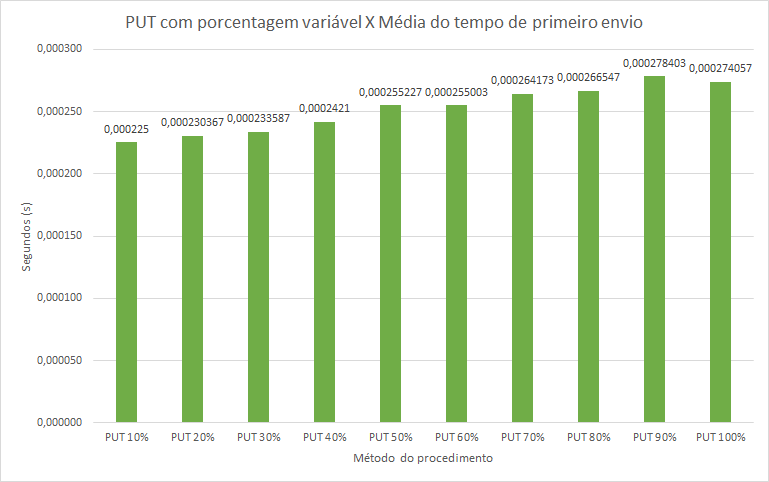
\includegraphics[width=.8\textwidth]{../imagens/PUTxPrimeiroEnvio}
	\caption{Tempo de envio}
	\label{fig:put_tempo_envio}
\end{figure}

\section{POST 1 tentativa}
No primeiro teste, conforme a figura \ref{fig:put_num_entregues},
será demonstrado o número de mensagens entregues, usando o tipo de mensagem POST, com porcentagens que variam de 10 a 100\%.
Esse teste simulará a taxa de entrega de um método PUT.

\begin{figure}[!htb]
	\centering
	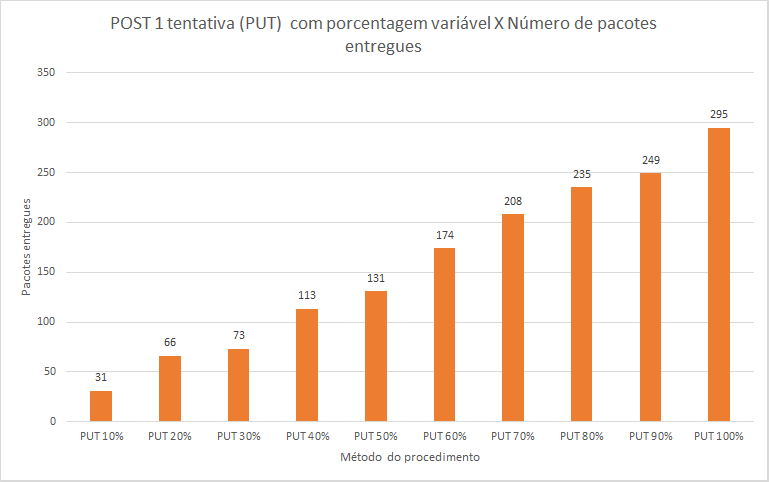
\includegraphics[width=.8\textwidth]{../imagens/PUTxNumentregues}
	\caption{Número de mensagens entregues}
	\label{fig:put_num_entregues}
\end{figure}

Como esperado, existe um ganho considerável de pacotes entregues, ao aumentar o parâmetro de porcentagem de entrega, variando praticamente na mesma proporção de pacotes entregues com a porcentagem definida no código.

\section{POST 5 tentativas}

O primeiro teste deste método, conforme figura \ref{fig:post_num_entregues}, mostra o número de mensagens do tipo POST entregues, segundo a variação da porcentagem de envio entre 10 a 100\%.
É importante lembrar que uma mensagem do tipo POST faz cinco tentativas de envio da mensagem.

\begin{figure}[!htb]
	\centering
	\includegraphics[width=0.8\textwidth]{../imagens/POSTxNumEntregues}
	\caption{Número de mensagens entregues}
	\label{fig:post_num_entregues}
\end{figure}
\hfill \break
\hfill \break
\hfill \break
\hfill \break
\hfill \break
\hfill \break
\hfill \break
\hfill \break
\hfill \break
\hfill \break

O segundo teste será o tempo de envio da primeira mensagem, para o método POST.

\begin{figure}[!htb]
	\centering
	\includegraphics[width=.8\textwidth]{../imagens/POSTxPrimeiroEnvio}
	\caption{Tempo de envio}
	\label{fig:post_tempo_envio}
\end{figure}

E por último, expõe-se o gráfico da média do tempo de recebimento do ACK para o método POST, na figura \ref{fig:post_media_tempo_ACK}.

\begin{figure}[!htb]
	\centering
	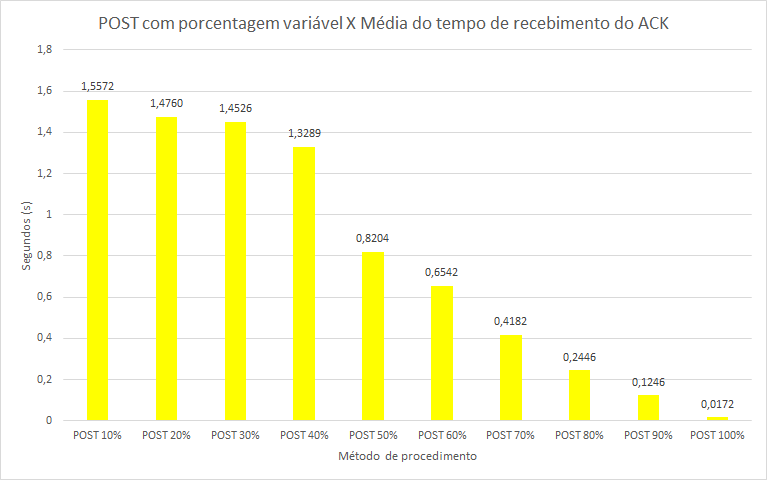
\includegraphics[width=.8\textwidth]{../imagens/POSTxMediatempopacoteentregue}
	\caption{Tempo de envio}
	\label{fig:post_media_tempo_ACK}
\end{figure}

\hfill \break
\hfill \break
\hfill \break

\section{Comparação de resultados}

Agora, passa-se às comparações dos métodos PUT e POST com uma tentativa, e POST com cinco tentativas.
A primeira comparação, feita na figura \ref{fig:num_entregues_post5_post1}, é entre o método POST com cinco tentativas e o método PUT, em relação ao número de mensagens entregues.

\begin{figure}[!htb]
	\centering
	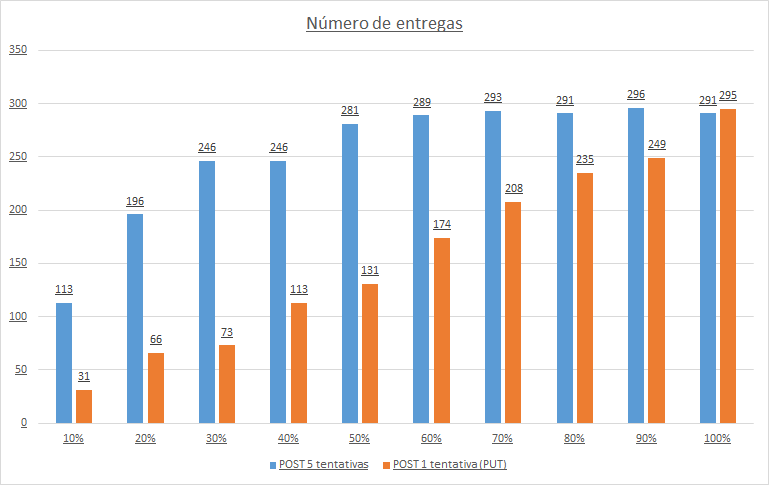
\includegraphics[width=.8\textwidth]{../imagens/Numero_entregas_PUTxPOST}
	\caption{Número de mensagens entregues}
	\label{fig:num_entregues_post5_post1}
\end{figure}

Como é observado, o número de mensagens entregues com cinco tentativas de entrega é muito superior em quase todos os testes; eles apenas se igualam quando a chance de entrega chega a 100\%. Isso comprova que, se a confiabilidade na entrega for fator importante, o aumento de tentativas de entrega é algo a se levar em conta. Em casos em que a taxa de entrega seja ainda inferior, é possível aumentar o número de tentativas de entrega para maior segurança.

Então, na figura \ref{fig:tempo_envio_1_msg_post5_put}, observa-se a comparação entre os métodos PUT e POST, para comparar o tempo gasto para envio da mensagem.

\begin{figure}[!htb]
	\centering
	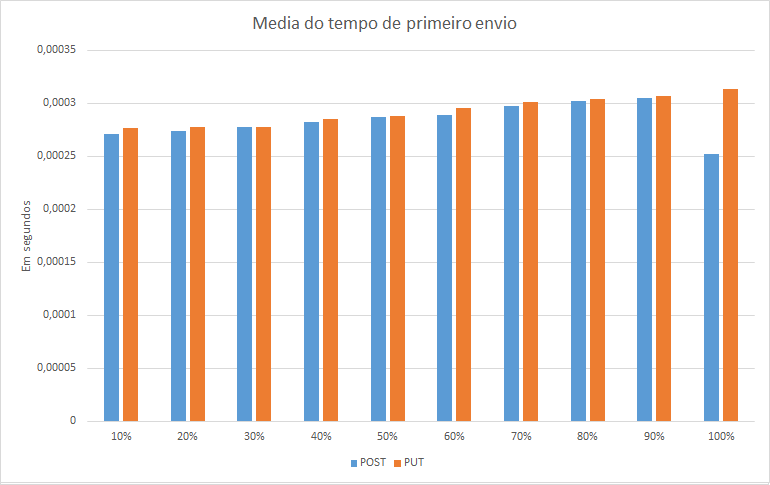
\includegraphics[width=.8\textwidth]{../imagens/media_primeiro_envio_PUTxPOST}
	\caption{Tempo de envio  da primeira mensagem}
	\label{fig:tempo_envio_1_msg_post5_put}
\end{figure}

Aqui é possível verificar a eficiência do método PUT, afinal, o tempo de execução é em média 10\% menor, já que este não precisa armazenar o dado enviado, pois é finalizado após o envio do programa, ao contrário do método POST, que ainda executa a função \texttt{buffer\_msg}, para achar uma posição em buffer e salvar a mensagem. Este método pode ser escolhido no caso de a perda de pacotes não ser tão relevante, ou, então, quando a taxa de entrega chegar próxima a 100\%.



\chapter{Conclusão}

Sistemas embarcados para controle e monitoração de ambientes têm ganhado seu espaço, com seu baixo custo, alta eficiência e possível aumento na produtividade e rendimento da tarefa onde eles são empregados.

Este trabalho teve a proposição do uso de um padrão novo, que é voltado para este tipo de situação, onde o hardware utilizado será o mais simples possível e a comunicação pode ter fatores que prejudiquem a entrega da mensagem, através de uma linguagem amplamente conhecida e que facilita a implementação neste tipo de sistema embarcado.

Ao final, chegou-se a um cliente e servidor relativamente simples e passíveis de serem alterados ou utilizados da forma que estão em embarcados de hardware mais modestos. Os resultados serviram para mostrar que, conforme a aplicação e o caso de uso, será possível escolher entre o método que mais se adequará ao projeto, tentando balancear taxa de entrega e tempo de execução.

Apesar de constar como objetivo inicial, não foi possível a implementação no hardware planejado. A principal razão para este problema foi uma alteração no funcionamento do sistema embarcado: inicialmente, ele havia sido planejado para enviar dados medidos, e, posteriormente, pensou-se em um método de alterar alguns parâmetros neste cliente. Tratando-se de uma aplicação que precisaria tanto receber parâmetros com comportamento de um servidor, quanto enviar parâmetros com comportamento de cliente, pensou-se em utilizar a biblioteca threads, porém, sistemas embarcados mais simples não possuem suporte para essa biblioteca, nem para outras bibliotecas similares.

\setlength{\baselineskip}{\baselineskip}

%%=============================================================================
%% Referências
%%=============================================================================
\bibliographystyle{abnt}
\bibliography{referencias/referencias}



%importante: Se precisar usar alguma seção ou subseção dentro dos apêndices ou
%anexos, utilizar o comando \tocless para não adicionar no Sumário
%Exemplos: 
% \tocless\section{Histórico}
%%=============================================================================
%% Apêndices
%%=============================================================================
\appendix
\chapter{C\'odigos do Cliente}
%iMPORTANTE: Se precisar usar alguma seção ou subseção dentro dos apêndices ou
%anexos, utilizar o comando \tocless para não adicionar no Sumário
%Exemplos: 
% \tocless\section{Histórico}
% \tocless\subsection{Detalhes}



\tocless\section{cli\_main.c}

\begin{lstlisting}

#include <stdlib.h>
#include <stdio.h>
#include <sys/types.h>
#include <sys/socket.h>
#include <netdb.h>
#include <time.h>
#include <netinet/in.h>
#include <arpa/inet.h>
#include <sys/ioctl.h>
#include <ctype.h>
#include <string.h>
#include <unistd.h>
#include "cli_main.h"

#define PORT 32012

#define PORCENTAGEM 100 /*DEFINE PORCENTAGEM DE MENSAGENS ENVIADAS*/

#define STRING_SERV 1
#define METHOD_PUT 1
#define METHOD_POST 0
#define METHOD_POST_PUT 0 /*Setado para testes de PUT (precisa ser setado junto com POST)*/

#define BILLION  1E9
#define SEC 3 /*SLEEP\_TIME*/
#define NSEC 5E8 /*SLEEP\_TIME*/

#define DEBUG 1
#define DEBUG_ID 0
#define DEBUG_ID_ARGS 0
#define DEBUG_ID_T 0
#define DEBUG_ID_OP 0
#define DEBUG_ID_P 0
#define DEBUG_ARG_H 0
#define DEBUG_CONT_MINUS 0
#define DEBUG_M_HEADER 0
#define DEBUG_ADD_HDR_TKL 0
#define DEBUG_ADD_OPTION 0
#define DEBUG_ADD_PAYLOAD 0
#define DEBUG_PARAMETROS 0
#define DEBUG_PRINT_HEADER 0
#define DEBUG_PRINT_TOKEN 0
#define DEBUG_PRINT_OPTION 0
#define DEBUG_PRINT_OPTION_M 0
#define DEBUG_PRINT_PAYLOAD 0
#define DEBUG_MONTA_OP 0
#define DEBUG_MONTA_H_T 0
#define DEBUG_SEPARA_STRING 0
#define DEBUG_SEND_MSG 0
#define DEBUG_SEND_MSG_BUFFER 0
#define DEBUG_MSG_RECEIVED 0
#define DEBUG_ARGS 0
#define DEBUG_PKT_ARG 0
#define DEBUG_PUT 0
#define DEBUG_VER_BUF 0
#define DEBUF_IMPRIMIR_BUF 0
#define DEBUG_TIMEOUT 0
#define DEBUG_TOKEN_SETADO 0
#define DEBUG_TIME_ALL 0
#define DEBUG_WHILE 0
#define DEBUG_PRINT_CLI_SERV 0
#define DEBUG_WHILE_ORDER 0

/*OPÇÕES*/
#define SAIR 1
#define TIME_CONTROL 1/*Se for sempre necessário calcular tempo*/
#define TOKEN_ALEATORIO 1
#define NUM_TIMEOUT 5   /*SE SELECIONAR 0, SE TORNA PUT (NAO TENTA REENVIAR)*/
#define NUM_DE_OPCOES 30
#define MAX_OPTIONS 10
#define MAX_TAMANHO_TOKEN 10 /*char*/
#define MAX_TAMANHO_OPTION 24 /*char*/
#define MAX_TAMANHO_PAYLOAD 64 /*char*/

#define ACK_WAIT_TIMEOUT_SEC 1
#define ACK_WAIT_TIMEOUT_USEC 0

#define MAX_LEN_OPTION 32
#define MAX_VALUE_OPTION 64
#define FUNC_ARG 0 /*Recebendo via argumentos no cmd*/
#define FUNC_STRINGS 1 /*Recebendo via strings digitadas*/


/*Definição de erros*/
#define erro_argumento_invalido 10
#define erro_argumento_token_invalido 11
#define erro_argumento_num_option_invalido 12
#define erro_argumento_payload_invalido 13
#define erro_argumento_mais_de_um_token 14
#define erro_argumento_mais_de_um_payload 15
#define erro_len_15 16
#define erro_len_invalida 17
#define erro_delta_15 18
#define erro_delta_invalida 19
#define erro_comando 20
#define erro_prim_arg_invalido 21
#define erro_seg_arg_invalido 22 
#define erro_payload_mais_ags 23
#define erro_payload_excede_tamanho 24
#define erro_option_excede_tamanho 25
#define erro_token_excede_tamanho 26
#define erro_buffer_cheio 27
#define erro_argumento_inv
#define erro_falta_argumento 30


void lida_erro_monta (short int erro);
void lida_erro_add (short int erro);
void lida_erro_send_msg (short int erro);

void printf_header (coap_header_t *hdr)
{
	printf("Header:\n");
	printf("  ver  0x%02X\n", hdr->ver);
	printf("  t    0x%02X\n", hdr->t);
	printf("  tkl  0x%02X\n", hdr->tkl);
	printf("  code 0x%02X\n", hdr->code);
	printf("  id   0x%02X%02X\n", hdr->id[0], hdr->id[1]);
}

void printf_token (coap_buffer_t *token)
{
	printf("Token:\n");
	printf("  size  0x%d\n",(int) token->len);
	printf("  token %s\n", token->p);
}
void printf_payload (coap_buffer_t *payload)
{
	printf("Payload:\n");
	printf("  size  0x%d\n",(int) payload->len);
	printf("  payload %s\n", payload->p);
}

void printf_option (coap_option_t *opt)
{
	printf("Option:\n");
	printf("  num  %d\n", (int)opt->num);
	printf("  num  0x%02x\n", opt->num);
	printf("  option buf len %d\n",(int) opt->buf.len);
	printf("  option buf p %s\n", opt->buf.p);
}

void printf_buffer(uint8_t *buffer)
{
	short int i;
	for (i=0; i<strlen((char *)buffer); i++)
	{
		printf("buffer [%d] = 0x%02x = %c\n", i, buffer[i], buffer[i]);
	}
}
void printf_buffer_m(uint8_t *buffer, short int size)
{
	short int i;
	for (i=0; i<size; i++)
	{
		printf("%02x ", buffer[i]);
	}
}
void printf_buffer_str(char buf[][512], int num_linhas)
{
	int i,j;
	for (i=0; i<num_linhas; i++)
	{		
		printf("\n");
		for (j=0; j<strlen(buf[i]); j++)
		{
			printf("0x%02X ", buf[i][j]);
		}
		printf("\n");
		printf("buffer [%d] = %s \n", i, (char *)buf[i]);
	}
}

void tempo_agora (char *tempo);
void get_time (struct timespec *time_now);
float calc_time_sub (struct timespec *start, struct timespec *stop);

void buffer_msg (char *buf_out, char *buf_out_p, short int *cont_msg, short int *pos, char buf_str[][512])
	{
		int k, m, ult_esc = -1;
#if DEBUG && DEBUG_SEND_MSG_BUFFER
		printf("buf_out send_msg = %s\n", buf_out);
#endif
	/*DECIDIR O QUE FAZER SE BUFFER ESTIVER CHEIO*/
	if(*cont_msg > 7)
	{
		lida_erro_send_msg (erro_buffer_cheio);
	}
	else
	{
#if DEBUG && DEBUG_SEND_MSG
		printf("123\n");
		printf("-2 0X%02X ", *(buf_out_p-2));
		printf("-1 0X%02X ", *(buf_out_p-1));
		printf(" 0X%02X ", *buf_out_p);
		printf("+1 0X%02X", *(buf_out_p+1));
		printf("\n");
		printf("strlen %d\n", strlen(buf_out));
		printf("printf ultima pos -2 = 0x%02X\n", buf_out[strlen(buf_out)-2]);
		printf("printf ultima pos -1 = 0x%02X\n", buf_out[strlen(buf_out)-1]);
		printf("printf ultima pos = 0x%02X\n", buf_out[strlen(buf_out)]);
		printf("printf ultima pos +1 = 0x%02X\n", buf_out[strlen(buf_out)]+1);
#endif
	
		buf_out_p = buf_out_p + strlen(buf_out);
		*buf_out_p++ = 0x20;
#if DEBUG && DEBUG_SEND_MSG
		printf("213\n");
		printf("-2 0X%02X ", *(buf_out_p-2));
		printf("-1 0X%02X ", *(buf_out_p-1));
		printf(" 0X%02X ", *buf_out_p);
		printf("+1 0X%02X", *(buf_out_p+1));
		printf("\n");
		printf("strlen %d\n", strlen(buf_out));
		printf("printf ultima pos -2 = 0x%02X\n", *(buf_out_p-2));
		printf("printf ultima pos -1 = 0x%02X\n", *(buf_out_p-1));
		printf("printf ultima pos = 0x%02X\n", *(buf_out_p));
		printf("printf ultima pos +1 = 0x%02X\n", *(buf_out_p+1));
#endif
	
#if DEBUG && DEBUG_SEND_MSG
		printf("321\n");
		printf("-2 0X%02X ", *(buf_out_p-2));
		printf("-1 0X%02X ", *(buf_out_p-1));
		printf(" 0X%02X ", *buf_out_p);
		printf("+1 0X%02X", *(buf_out_p+1));
		printf("\n");
		printf("strlen %d\n", strlen(buf_out));
		printf("printf ultima pos -2 = 0x%02X\n", buf_out[strlen(buf_out)-2]);
		printf("printf ultima pos -1 = 0x%02X\n", buf_out[strlen(buf_out)-1]);
		printf("printf ultima pos = 0x%02X\n", buf_out[strlen(buf_out)]);
		printf("printf ultima pos +1 = 0x%02X\n", buf_out[strlen(buf_out)]+1);
#endif
#if DEBUG && DEBUG_SEND_MSG
		printf("\n");
		printf("buf_out = %s, buf_out len = %d, buf_out size = %d\n", buf_out, strlen((char*)buf_out), sizeof(buf_out));
	for (m = 0; m<(int)strlen((char*)buf_out); m++)
	{
		printf("buf[%d]= 0x%02X\n", m, buf_out[m]);
	}
		printf("\n");
	for (m = 0; m<(int)strlen((char*)buf_out); m++)
	{
		printf("%02X ", buf_out[m]);
	}
		printf("\n");
#endif
	
#if DEBUG && DEBUG_SEND_MSG
		printf("rsplen = %d\n", (int) rsplen);
#endif
	
		k=1;
	while(k==1)
	{
#if DEBUG && DEBUG_SEND_MSG
		printf("ult_esc = %d", ult_esc);
#endif
	for (m = 0; m<8; m++)
	{
#if DEBUG && DEBUG_VER_BUF
		printf("pos [%d] = %d\n", m, pos[m]);
#endif
	}
	if(ult_esc == 7)
	{
		ult_esc = -1;
	}
	if(pos[ult_esc+k]==0)
	{
#if DEBUG && DEBUG_SEND_MSG
		printf("Ult_esc = %d, cont_msg = %d, pos[ult_esc] = %d\n", ult_esc, *cont_msg, pos[ult_esc+k]);
#endif
		ult_esc++;
		*cont_msg = *cont_msg + 1;;
		pos[ult_esc] = 1;
		memcpy(buf_str[ult_esc], buf_out, 512);
		k++;
#if DEBUG && DEBUG_SEND_MSG
		printf("buf = %s \n", (char*)buf_str[ult_esc]);
		printf("cont_msg = %d\n", *cont_msg);
#endif
		break;
	}
	ult_esc++;
	
	}
}

int lida_msg_recebida (char *buf_in, char buf_str[][512], short int *cont_msg, short int *pos, struct timespec *time_post, struct timespec *time_start, FILE *pFile)
{
	int i, j;
	float time_calc = 0;
#if DEBUG && DEBUG_MSG_RECEIVED
	printf("\nbuf_in = %s\n", buf_in);
	for (i=0; i<strlen(buf_in); i++)
	{
		printf("0x%02X ", (uint8_t) buf_in[i]);
	}
	printf("\n");
	for (i=0; i<strlen(buf_in); i++)
	{
		printf("%c ",buf_in[i]);
	}
	for (i=0; i<8; i++)
	{
	
		printf("\npos [%d] = %d,", i, pos[i]);
		printf("buf_str [%d] = ", i);
		printf_buffer_m((uint8_t *)buf_str[i], 9);
		
		printf("\ncont_msg = %d\n", *cont_msg);
	#endif
	for (i=0; i<8; i++)
	{
		if (pos[i] == 1)
		{
#if DEBUG && DEBUG_MSG_RECEIVED
			printf("buf_in[%d] = 0x%02X\n", i, buf_in[0]);
			printf("buf_str[%d] = 0x%02X\n", i, buf_str[0][0]);
			printf("buf_in[%d] = 0x%02X\n", i+1, buf_in[1]);
			if ((buf_in[1] & 0xFF)== 0x84)
			{
				printf("É igual\n");
			}
			else
			{
				printf("Não é igual\n");
			}
			printf("buf_str[%d] = 0x%02X\n", i+1, buf_str[0][1]);
#endif
			
#if METHOD_POST									/*Resposta(6)*/			
			if (((buf_in[0] & (0xF0)) == 0x60) && ((buf_in[0] & 0X0F) == (buf_str[i][0] & 0x0F)) && ((buf_in[1] & 0xFF )== 0x44))
			#endif
#if METHOD_PUT
			if (((buf_in[0] & (0xF0)) == 0x60) && ((buf_in[0] & 0X0F) == (buf_str[i][0] & 0x0F)) && ((buf_in[1] & 0xFF )== 0x44))
#endif
			{
				int cont = 0;
				for (j=0; j<(buf_in[0] & 0x0F); j++)
				{
#if DEBUG && DEBUG_MSG_RECEIVED
					printf("entrando no for buf_in\n");
					printf("j = %d\n", j);
#endif
					if(buf_in[2+j] == buf_str[i][2+j])
					{
#if DEBUG && DEBUG_MSG_RECEIVED
						printf("buf_in = 0x%02X, buf_str = 0x%02X\n", buf_in[2+j], buf_str[i][2+j]);
#endif
						cont++;
					}
				}
				if (cont == (buf_in[0] & 0x0F))
				{
					printf("Mensagem ACK recebida, buffer limpo\n");
#if TIME_CONTROL
					get_time(time_post);
					
#if DEBUG_TIME_ALL
					printf("time_start.sec = %d, time_start.nsec = %d\ntime_post_ACK.sec = %d, time_post_ACK.nsec = %d", (int)time_start->tv_sec, (int)time_start->tv_nsec, (int)time_post->tv_sec, (int)time_post->tv_nsec);
#endif
					time_calc = calc_time_sub (time_start, time_post);	    		
					printf( "\nHow long to receive ACK in a POST request = %lf\n", time_calc);
					if(pFile!=NULL)
					{
						fprintf(pFile, "%lf,", time_calc);
						fprintf(pFile, "Y;\n");
					}
#endif
					
					pos[i] = 0;
					*cont_msg = *cont_msg - 1;
					memset(buf_str[i], 0x00, 512);
					return 1;
				}
			}
			else
			{
				printf("Mensagem não é ACK, mensagem incorreta\n");
				return 0;
			}
		}
	}
	return 0;
}

void tempo_agora (char *tempo)
{
	time_t  t= time(NULL);
	struct tm tm = *localtime(&t);
	snprintf(tempo,42," Hora: ""%d"":""%d"":""%d" " ""Data:""%d""/""%d", tm.tm_hour, tm.tm_min, tm.tm_sec, tm.tm_mday, tm.tm_mon);
	printf("Tempo agora = %s\n", tempo);
}

void get_time (struct timespec *time_now)
{
	if( clock_gettime( CLOCK_REALTIME, time_now) == -1 )
	{
		perror( "clock gettime" );
		exit( EXIT_FAILURE );
	}
}
float calc_time_sub (struct timespec *start, struct timespec *stop)
{
	float tempo_decorrido;
	tempo_decorrido = ( stop->tv_sec - start->tv_sec )
	+ ( stop->tv_nsec - start->tv_nsec )
	/ BILLION;
	return tempo_decorrido;
}


void n_sleep (struct timespec *sleep_time)
{
	if(nanosleep(sleep_time, NULL) < 0)   
	{
		printf("Nano sleep system call failed \n");
		exit (0);
	}
}

/*Recebendo mensagem com 00 00, cliente interpreta restante como 0, porém vem payload após 00 00*/
short int corrige_len (uint8_t *buffer, short int size)
{
	short int i = 0;
	short int cont_ff = 0;
	while (i<size && (cont_ff<1 || buffer[i] != 0x00))
	{
		if(buffer[i] == 0xff)
		{
			cont_ff++;
		}
		printf("buffer[%i] = %c\n", i, buffer[i]);
		i++;
	}
	return i;
}
void monta_pkt (coap_packet_t *pkt, uint8_t *buf)
{
	uint8_t *p = NULL;
	uint16_t running_delta = 0;
	
	/*max len = 16*/
	/*max delta = 64*/
	
	/*Adicionar tempo ao final do pacote*/
	char tempo[100];
	tempo_agora(tempo);
	/*Precisei diminuir o tamanho do restante da mensagem, erro "stack smashing detected"*/
	
	
	
	short int i=0;
	buf[0] = (pkt->hdr.ver & 0x03) << 6;
	buf[0] |= (pkt->hdr.t & 0x03) << 4;
	buf[0] |= (pkt->hdr.tkl & 0xFF);
	buf[1] = pkt->hdr.code;
	buf[2] = pkt->hdr.id[0];
	buf[3] = pkt->hdr.id[1];
	p = buf+4;
	memcpy(p, pkt->tok.p, pkt->hdr.tkl);
	p = p+pkt->hdr.tkl;
	short int aux = (short int)pkt->numopts;
	for (i=0; i<aux; i++)
	{
#if DEBUG && DEBUG_MONTA_OP
		printf("Entrando no for\n");
#endif
#if DEBUG && DEBUG_PRINT_OPTION_M
		printf_option(&pkt->opts[i]);
#endif
		uint8_t len = pkt->opts[i].buf.len;
		uint8_t delta = (int)pkt->opts[i].num;
		uint8_t op_num_len = 0;
		delta = delta - running_delta;
		running_delta = 2*running_delta + delta;
		uint8_t len_aux = 0, delta_aux = 0;
		/*Lida com opções, RFC7252, Página 18*/
		if(delta>13 && delta<65)
		{
			delta_aux = delta-13;
			delta = 13;
		}
		else if (delta == 15)
		{
			lida_erro_monta(erro_delta_15);
		}
		else if (delta < 0 || delta >= MAX_VALUE_OPTION) /*-> MAX_VALUE_OPTION = 64*/
		{
			lida_erro_monta (erro_delta_invalida);
		}
		
		/*Lida com opções, RFC7252, Página 19*/
		if(len>13 && len<17)
		{
			len_aux = len-13;
			len = 13;
		}
		else if (len == 15)
		{
			lida_erro_monta(erro_len_15);
		}
		else if (len < 0 || len >= MAX_LEN_OPTION) /*-> MAX_LEN_OPTION = 16*/
		{
			lida_erro_monta (erro_len_invalida);
		}
		
		
#if DEBUG && DEBUG_MONTA_OP
		printf("Conteudo de opts[%d]->num = %d\n", i, (int)pkt->opts[i].num);
		printf("Conteudo de opts[%d]->num = 0x%02x\n", i, pkt->opts[i].num);
		printf("Conteudo de delta = %d\n", (int)delta);
		printf("Conteudo de delta = 0x%02x\n", delta);
		printf("Conteudo de delta_aux = %d\n", (int)delta_aux);
		printf("Conteudo de delta_aux = 0x%02x\n", delta_aux);
		printf("Conteudo de running_delta = %d\n", (int)running_delta);
		printf("Conteudo de running_delta = 0x%02x\n", running_delta);
		printf("Conteudo de opts[%d]->buf.len = %d\n", i, pkt->opts[i].buf.len);
		printf("Conteudo de opts[%d]->buf.p = %s\n", i, (char *) pkt->opts[i].buf.p);
#endif
		
#if DEBUG && DEBUG_MONTA_OP
		printf("Conteudo de op = %d\n", delta);
#endif
		op_num_len = (0xFF & (delta << 4 | len));
#if DEBUG && DEBUG_MONTA_OP
		printf("antes do *p\n");
#endif
		*p++ = op_num_len;
		if(delta==13)
		{
#if DEBUG && DEBUG_MONTA_OP
			printf("Entrando no delta == 13\n");
#endif
			*p++=delta_aux;
#if DEBUG && DEBUG_MONTA_OP
			printf("p = %c, 0x%02X, p[-1] = %c, 0x%02X\n", *p, *p, *(p-1),*(p-1));
#endif
		}
		if(len == 13)
		{
			*p++=len_aux;
		}
		memcpy(p, pkt->opts[i].buf.p, pkt->opts[i].buf.len);
		p = p + pkt->opts[i].buf.len;
	}
	/*Payload*/
	
	*p++ = 0xFF;
	memcpy(p, pkt->payload.p, pkt->payload.len);
	p = p+pkt->payload.len;
	
	/*Adicionando tempo*/
	memcpy(p, tempo, (int)strlen(tempo));
	p=p+(int)strlen(tempo);

}

void monta_header_token (coap_packet_t *pkt, uint8_t *token)
{
	/*0100 0000 0000 0011 0000 0010 0000 0001*/
	pkt->hdr.ver = 	 0x01; /* versão 01;*/
	pkt->hdr.t = 	 0x00; /* code 0 (confirmable);*/
	/*pkt->hdr.tkl = 	 0x00; /*Tamanho do token -> para testes, 0*/
#if METHOD_POST
	pkt->hdr.code =  0x02; /*request -> 0000 0010 -> POST*/
#endif
#if METHOD_PUT
	pkt->hdr.code =  0x03; /*request -> 0000 0011 -> PUT*/
#endif
#if METHOD_POST_PUT
	pkt->hdr.code =  0x03; /*request -> 0000 0011 -> PUT*/
#endif
	/* GERANDO id aleatoriamente*/
	srand(time(NULL));
	short int var_aux = rand()%254;
	pkt->hdr.id[0] = (uint8_t) var_aux; /*0010 -> TESTE*/
	var_aux = rand()%254;
	pkt->hdr.id[1] = (uint8_t) var_aux; /*0001 -> TESTE*/
	/* GERANDO TOKEN aleatoriamente*/
#if TOKEN_ALEATORIO
	var_aux = rand()%254;
	token[0] = var_aux;
#endif
#if DEBUG && DEBUG_MONTA_H_T
	printf("token = %d, var_aux = %d\n", token[0], var_aux);
#endif
#if TOKEN_ALEATORIO
	var_aux = rand()%254;
	token[1] = var_aux;
	#endif
#if DEBUG && DEBUG_MONTA_H_T
	printf("token = %d, var_aux = %d\n", token[1], var_aux);
#endif
#if TOKEN_ALEATORIO
	var_aux = rand()%254;
	token[2] = var_aux;
#endif
#if DEBUG && DEBUG_MONTA_H_T
	printf("token = %d, var_aux = %d\n", token[2], var_aux);
#endif
#if TOKEN_ALEATORIO
	var_aux = rand()%254;
	token[3] = var_aux;
#endif
#if DEBUG && DEBUG_MONTA_H_T
	printf("token = %d, var_aux = %d\n", token[3], var_aux);
#endif
#if TOKEN_ALEATORIO
	var_aux = rand()%254;
	token[4] = var_aux;
#endif
#if DEBUG && DEBUG_TOKEN_SETADO
	token[0] = 0x30;
	token[1] = 0x31;
	token[2] = 0x32;
	token[3] = 0x33;
	token[4] = 0x34;
#endif
#if DEBUG && DEBUG_MONTA_H_T
	printf("token = %d, var_aux = %d\n", token[4], var_aux);
#endif
	pkt->tok.p = token;
	pkt->tok.len = 5;
	pkt->hdr.tkl = pkt->tok.len;
	
#if DEBUG && DEBUG_M_HEADER
	printf_header(&pkt->hdr);
#endif
}

void cria_pkt (coap_packet_t *pkt, uint8_t *token)
{
	monta_header_token (pkt, token);
	pkt->numopts = 0;
}
void add_payload (coap_packet_t *pkt, char *payload)
{
	if (strlen(payload) > 64)
	{
		lida_erro_add(erro_payload_excede_tamanho);
	}
	else
	{
		pkt->payload.len = strlen(payload);
		pkt->payload.p = (uint8_t *)payload;
#if DEBUG && DEBUG_PRINT_PAYLOAD
		printf_payload(&pkt->payload);
#endif
}

}
void add_option (coap_packet_t *pkt, short int cont_aux, short int *buf_aux_opt_n, char *op_conteudo, short int numopt, short int *option_running_delta)
{
	short int num_op = *buf_aux_opt_n;
	if (strlen(op_conteudo) > 24)
	{
		lida_erro_add(erro_option_excede_tamanho);
	}
	else
	{
#if DEBUG && DEBUG_ADD_OPTION
		printf("Option num, antes do delta = %d\n", num_op);
#endif
#if DEBUG && DEBUG_ADD_OPTION
		printf("Option running delta = %d\n", *option_running_delta);
#endif
#if DEBUG && DEBUG_ADD_OPTION
		printf("Option num - option_running_delta = %d\n", num_op);
#endif
		*buf_aux_opt_n = num_op;
		pkt->opts[cont_aux].num = *buf_aux_opt_n;
		pkt->opts[cont_aux].buf.len = strlen(op_conteudo);
		pkt->opts[cont_aux].buf.p = (uint8_t *) op_conteudo;
#if DEBUG && DEBUG_PRINT_OPTION
		printf_option(&pkt->opts[cont_aux]);
#endif
	}
}
void add_token_hdr_tkl (coap_packet_t *pkt, char *token)
{
	/*HDR_TKL*/
	short int tkl;
	tkl = strlen(token);
	if (tkl > MAX_TAMANHO_TOKEN)
	{
		lida_erro_add(erro_token_excede_tamanho);
	}
	else
	{
		pkt->hdr.tkl = tkl;
#if DEBUG && DEBUG_PRINT_HEADER
		printf_header(&pkt->hdr);
#endif
	/*HDR_TKL*/
		pkt->tok.len = strlen (token);
		pkt->tok.p = (uint8_t *)token;
#if DEBUG && DEBUG_PRINT_TOKEN
		printf_token(&pkt->tok);
#endif
	}
}
void lida_erro_send_msg (short int erro)
{
	if(erro == erro_buffer_cheio)
	{
		printf("Buffer cheio, erro %d\n", erro);
	}
	exit (0);
}
void lida_erro_add (short int erro)
{
	if (erro == erro_token_excede_tamanho)
	{
		printf("Token excede tamanho máximo %d\n", erro);
	}
	else if (erro == erro_option_excede_tamanho)
	{
		printf("Option excede tamanho máximo %d\n", erro);
	}
	else if (erro == erro_payload_excede_tamanho)
	{
		printf("Payload excede tamanho máximo %d\n", erro);
	}
	exit (0);
}

void lida_erro_monta (short int erro)
{
	if (erro == erro_len_15)
	{
		printf("Len = 15, numero reservado, erro %d\n", erro);
	}
	else if (erro == erro_len_invalida)
	{
		printf("Len invalido, numero reservado, erro %d\n", erro);
	}
	else if (erro == erro_delta_15)
	{
		printf("Delta = 15, numero reservado, erro %d\n", erro);
	}
	else if (erro == erro_delta_invalida)
	{
		printf("Delta inválido, numero reservado, erro %d\n", erro);
	}
	exit (0);
}
void lida_erro_id(short int erro, short int argc, char **argv)
{
	if(erro == erro_argumento_invalido)
	{
		printf("Recebendo argumento(s) inválido(s) GERAL, erro %d\n", erro);
	}
	else if(erro == erro_prim_arg_invalido)
	{
		printf("Recebendo primeiro argumento inválido, erro %d\n", erro);
	}
	else if(erro == erro_seg_arg_invalido)
	{
		printf("Recebendo segundo argumento inválido, erro %d\n", erro);
	}
	else if(erro == erro_argumento_token_invalido)
	{
		printf("Recebendo argumento no token inválido, erro %d\n", erro);
	}
	else if(erro == erro_argumento_num_option_invalido)
	{
		printf("Recebendo argumento num option inválido, erro %d\n", erro);
	}
	else if(erro == erro_argumento_payload_invalido)
	{
		printf("Recebendo argumento no payload inválido, erro %d\n", erro);
	}
	else if(erro == erro_argumento_mais_de_um_token)
	{
		printf("Recebendo mais de um token, erro %d\n", erro);
	}
	else if(erro == erro_argumento_mais_de_um_payload)
	{
		printf("Recebendo mais de um payload, erro %d\n", erro);
	}
	else if(erro == erro_payload_mais_ags)
	{
		printf("Recebendo payload mais de um argumento, erro %d\n", erro);
	}
	else if(erro == erro_falta_argumento)
	{
		printf("Recebendo poucos argumentos, erro %d\n", erro);
	}
	else if(erro == erro_comando)
	{
		printf("Recebendo comando invalido, erro %d\n", erro);
	}
	short int i;
	printf("Mensagem enviada: \n");
	for (i=1; i<argc; i++)
	{
		printf("%s ", argv[i]);
	}
	printf("\n");
	exit (0);
}

short int veri_token (char *argv1)
{
	short int i;
	for (i=0; i<strlen(argv1); i++)
	{
		/*ASCII 48-57*/
		if (argv1[i] < 48 || (argv1[i] > 57 && argv1[i] < 65) || (argv1[i] > 90 && argv1[i] < 97) || argv1[i] > 122)
		{
			return 1;
		}
	}
	return 0;
}

short int veri_option (char *argv1, char *argv2)
{
	short int i;
	short int cont = 0;
	for (i=0; i<strlen(argv1); i++)
	{
		/*ASCII 48-57*/
		if (argv1[i] < 48 || argv1[i] > 57)
		{
			return 1;
		}
	}
	if(cont > 0)
		return 1;
	else
		return 0;
}

short int veri_payload (char *argv1)
{
	short int i;
	if (argv1[0] == 43 || argv1[0] == 45)
	return 1;
	for (i=1; i<strlen(argv1); i++)
	{
		/*ASCII 48-57*/
		if (argv1[i] < 48 || (argv1[i] > 57 && argv1[i] < 65) || (argv1[i] > 90 && argv1[i] < 97) || argv1[i] > 122)
		{
			return 1;
		}
	}
	return 0;
	}
	
short int find_minus_plus (char *argv)
{
	if (argv[0] == '-' || argv[0] == '+')
	{
		return 1;
	}
	return 0;
}


void identifica_arg (coap_packet_t *pkt, int argc, char **argv, char *buf_aux_opt_c, short int *buf_aux_opt_n)
{
	short int j;
	char *end;
	short int cont_p = 0; /* Mesma coisa do Token abaixo*/
	short int cont_op = 0; /* Mesma coisa do Token abaixo*/
	short int cont_t = 0; /* Apenas um token, caso cont_t > 1 erro de argumento;*/
	short int option_delta = 0; /*Option running delta*/
#if DEBUG_ID && DEBUG_ID_ARGS
	for (j=1; j<argc; j++)
	{
		printf("argc = %d, j = %d\n", argc, j);
		printf("args = %s\n", argv[j]);
	}
#endif
	
	j = 1;
	if (argc <3)
	#endif
	{
		lida_erro_id(erro_falta_argumento,argc, argv);
	}
	else if (0 != strcmp(argv[0],"cliente") && 0 != strcmp(argv[0],"cli"))
	{
		lida_erro_id(erro_prim_arg_invalido,argc, argv);
	}
	else if (0 != strcmp(argv[1], "-t") && 0 != strcmp(argv[1], "-op"))
	{
		lida_erro_id(erro_seg_arg_invalido, argc, argv);
	}
	while (j<argc)
	{
#if DEBUG && DEBUG_ID
		printf("argv[%d] = %s, argc = %d, j = %d\n", j, argv[j], argc, j);
		printf("j = %d\n", j);
#endif
		if(strcmp(argv[j], "-t") == 0)
		{
#if DEBUG_ID_T && DEBUG
			printf("entrando no -t \n");
#endif
			cont_t++;
			if (cont_t > 1)
			{
				lida_erro_id(erro_argumento_mais_de_um_token, argc, argv);
			}
			/*TODO posso especificar esse erro também*/
			else if (j+2 > argc)
			{
				lida_erro_id(erro_argumento_token_invalido, argc, argv);
			}
			/*TODO posso dividir esse if para ter mais detalhes do meu erro;*/
			else if(veri_token(argv[j+1]))
			{
				lida_erro_id(erro_argumento_token_invalido, argc, argv);
			}
			else
			{
				
#if DEBUG_ID_T && DEBUG
				printf("1t)argv[j] = -t\n");
				printf("2t)argv[j] = %s, ", argv[j]);
				printf("3t)argv[j+1] = %s\n", argv[j+1]);
				printf("4t) j = %d\n", j);
#endif
				add_token_hdr_tkl(pkt, argv[j+1]);
				j+=2;
			}
		}
		else if(strcmp(argv[j], "-op") == 0)
		{
			cont_op++;
			pkt->numopts++;
			short int cont_aux = cont_op - 1;
			/*TODO posso especificar esse erro também
			if (j+3 > argc)
			{
				lida_erro_id(erro_argumento_num_option_invalido, argc, argv);
			}
			else if(veri_option (argv[j+1], argv[j+2]))
			{
				lida_erro_id(erro_argumento_num_option_invalido, argc, argv);
			}
			else
			{
				/*Converte string option para inteiro;*/
				buf_aux_opt_n[cont_op-1] = strtol(argv[j+1], &end, 0);
#if DEBUG_ID_OP && DEBUG
				printf("1op)argv[j] = -op\n");
				printf("2op)argv[j] = %s, ", argv[j]);
				printf("3op)argv[j+1] = %s\n", argv[j+1]);
				printf("4op) j = %d\n", j);
#endif
				add_option(pkt, cont_aux, &buf_aux_opt_n[cont_op-1], argv[j+2], cont_op, &option_delta);
				j+=3;
			}
		}
		else if(strcmp(argv[j], "-p") == 0)
		{
			cont_p++;
			/*TODO posso especificar esse erro também*/
			if (j+2 > argc)
			{
				printf("Nao existe arg\n");
				lida_erro_id(erro_argumento_payload_invalido, argc, argv);
			}
			/*TODO mesmo do TOKEN, dividir para especificar*/
			else if(cont_p > 1)
			{
				printf("Mais de um payload\n");
				lida_erro_id(erro_argumento_payload_invalido, argc, argv);
			}
			else
			{
			
#if DEBUG_ID_P && DEBUG
				printf("1p)argv[j] = -p\n");
				printf("2p)argv[j] = %s, ", argv[j]);
				printf("3p)argv[j+1] = %s\n", argv[j+1]);
				printf("4p) j = %d\n", j);
#endif
				add_payload(pkt, argv[j+1]);
				j+=2;
			}
		}
		else if (cont_p > 0)
		{
			lida_erro_id(erro_payload_mais_ags, argc, argv);
		}
		else if(cont_p == 0 && cont_op == 0)
		{
			lida_erro_id (erro_comando, argc, argv);
		}
		}
}

void separa_string (char **string_sep, char *buf, short int n_str, short int len)
{
	short int i;
	short int count_w = 0, j = 0;
	for (i=0; i<len; i++)
	{
#if DEBUG && DEBUG_SEPARA_STRING
		printf("buf[%d] = %c\n", i, buf[i]);
		printf ("Count_w = %d, j = %d, i = %d\n", count_w, j, i);
#endif
		if (buf[i] == ' ')
		{
		
			string_sep[count_w][j] = '\0';
			count_w++;
			j=0;
		}
		else
		{
			string_sep[count_w][j] = buf[i];
			j++;
		}
	}
#if DEBUG && DEBUG_SEPARA_STRING
	printf("String 1 = %s\n", string_sep[0]);
	printf("String 2 = %s\n", string_sep[1]);
	for (i=0; i<n_str; i++)
	{
		printf("1)String %d = %s\n", i, string_sep[i]);
	}
#endif
	}
short int  conta_espc (char *buf)
{
	short int i, cont=0;
	if (buf[0] == ' ')
	{
		printf("Erro\n");	
	}
	for (i=0; i<strlen(buf); i++)
	{
		if((buf[i] == ' ' && buf[i-1] != ' ')|| buf[i] == 0x0a)
		{
			cont++;
		}
	}
	return cont;
}

#if DEBUG && DEBUG_PKT_ARG
int main (int argc, char *argv[])
#endif
#if FUNC_STRINGS
int main_cli ()
#endif
{
#if DEBUG && DEBUG_PKT_ARG
#endif
	/*Tempo*/
	struct timespec time_start; /*Só para não precisar alterar a função lida_msg*/
	
#if METHOD_POST
	#if METHOD_POST_PUT
		struct timespec time_put;
	#else
		struct timespec time_post, time_resend, time_post_send;	
#endif
#else
	#if METHOD_PUT
		struct timespec time_put;
#endif
#endif
#if TIME_CONTROL
	get_time(&time_start);
#endif
	
	/*memset(pkt, 0, sizeof(pkt));*/
	/*Salvar logs em txt*/
	FILE * pFile;
	time_t t = time(NULL);
	struct tm tm = *localtime(&t);
	char date[50];
#if METHOD_PUT
	snprintf(date,50, "Dia=%d_Metodo=PUT_Porcentagem=%d",tm.tm_mday, PORCENTAGEM);
#else
	#if METHOD_POST
		#if METHOD_POST_PUT
			snprintf(date,50, "Dia=%d_Metodo=PUT_Porcentagem=%d",tm.tm_mday, PORCENTAGEM);
		#else
			snprintf(date,50, "Dia=%d_Metodo=POST_Porcentagem=%d",tm.tm_mday, PORCENTAGEM);
		#endif	
	#endif
#endif
	pFile = fopen (date,"a+");
	/*VARIAVEL ALEATORIA DE ENVIO
	srand (time(NULL)); /*RANDOM FUNCTION*/
	
	/*CONEXAO*/
	int fd;
	
	struct sockaddr_in cliaddr;
	fd = socket(AF_INET,SOCK_DGRAM,0);
	bzero(&cliaddr,sizeof(cliaddr));
#if METHOD_POST
	socklen_t szcliaddr = sizeof(cliaddr);
#endif
	cliaddr.sin_family = AF_INET;
	cliaddr.sin_addr.s_addr = inet_addr("192.168.0.103");
	cliaddr.sin_port = htons(32011);
	bind(fd,(struct sockaddr *)&cliaddr, sizeof(cliaddr));
	
	/*TIMEOUT*/
#if METHOD_POST	
	char buf_str[8][512];
	struct timeval tv;
	tv.tv_sec = ACK_WAIT_TIMEOUT_SEC;
	tv.tv_usec = ACK_WAIT_TIMEOUT_USEC;
	#if METHOD_POST_PUT
	#else
		short int num_timeouts = 0;
	#endif
#endif
	printf("\n");
	char buf_in[512], buf_out[512];
	char string_aux[50];
	/*Mensagem enviada*/
	strncat(string_aux, "cli -op 11 var -op 11 temperature -p 0810D",50);
	int str_len = strlen(string_aux);
	string_aux[str_len] = '\n';
	string_aux[str_len+1] = '\0';
#if DEBUG && DEBUG_VER_BUF
	char op[3];
#endif
	/*Variável utilizada para salvar tempo de envio;*/
	float time_calc = 0;
	/*Fim de argumentos*/
	
	
#if METHOD_POST
	short int cont_msg = 0;
	short int pos[8] = {0, 0, 0, 0, 0, 0, 0, 0};
#endif
	/*Mensagem*/
	/*buffer*/
	coap_packet_t pkt3;
	uint8_t token[5];
	cria_pkt(&pkt3, token);
	memset(buf_out, 0x00, 512);
	memset(buf_in, 0x00, 512);
#if METHOD_POST
	#if METHOD_POST_PUT
	#else
		num_timeouts = 0;
	#endif
#endif
	
#if STRING_SERV
	strncat(buf_out, string_aux, 511);				
	#if DEBUG && DEBUG_PRINT_CLI_SERV 
		printf_buffer((uint8_t *)buf_out);
	#endif
#else 
	fflush(stdin);
	printf("Digite a mensagem:\n");
	fgets(buf_out, 512, stdin);
	get_time(&time_start); /*Tempo -> Após digitar mensagem*/
	#if DEBUG && DEBUG_PRINT_CLI_SERV 
	printf_buffer((uint8_t *)buf_out);
	#endif
#endif
	
#if METHOD_POST
	char *buf_out_p = buf_out;
#endif
	
	short int i;
	char buf_aux_opt_c2[60] = "";
	short int buf_aux_opt_n2[10];
	
	short int len = strlen(buf_out)-1;
	short int n_str = conta_espc (buf_out);
	char **string_sep;
	string_sep = malloc(n_str * sizeof(char*));
	for (i = 0; i<n_str; i++)
		string_sep[i] = malloc((20) * sizeof(char));
	
#if DEBUG && DEBUG_SEPARA_STRING
	printf("Buffer_in = %s\nLen = %d\nNumero de Strings = %d\n", buf_out, len, n_str);
#endif
	separa_string(string_sep, buf_out, n_str, len);
	
	identifica_arg (&pkt3, n_str, string_sep, buf_aux_opt_c2, buf_aux_opt_n2);
#if SAIR /*Utilizada para testes, se receber a mensagem sair, sai do programa*/	
	if(0 == strcmp(buf_out, "sair\n\0"))
	{
		printf("Saindo 2\n");
		sendto(fd, "sair", (size_t)6, 0, (struct sockaddr *) &cliaddr, sizeof(cliaddr));
		close(fd);
		return 0;
	}
#endif
	memset(buf_out, 0x00, 512);
	monta_pkt(&pkt3, (uint8_t *)buf_out);
	
	printf("Mensagem enviada:\n");
	printf_buffer_m ((uint8_t *)buf_out, strlen(buf_out));
	size_t rsplen = strlen(buf_out);
#if DEBUG && DEBUG_SEND_MSG
	printf("buf_out [0] = %c, 0x%02X", *buf_out_p, *buf_out_p);
#endif
	printf("\n");
	printf("Buffer_out = %s\n", buf_out);
#if DEBUG && DEBUG_SEND_MSG
	printf("cont_msg = %d\n",cont_msg);
#endif
	
#if METHOD_POST
	if (rand()%100<PORCENTAGEM)
	{
		printf("\n\nSending\n\n");
		sendto(fd, buf_out, rsplen, 0, (struct sockaddr *) &cliaddr, sizeof(cliaddr));
	}
	else
	{
		printf("\n\nNot sending, simulando erro de comunicação\n\n");
	}
#if METHOD_POST_PUT
#else
	buffer_msg (buf_out, buf_out_p, &cont_msg,  pos, buf_str);
#endif
#else
	#if METHOD_PUT
		if (rand()%100<PORCENTAGEM)
		{
			printf("\n\nSending\n\n");
			sendto(fd, buf_out, rsplen, 0, (struct sockaddr *) &cliaddr, sizeof(cliaddr));
		}
		else
		{
			printf("\n\nNot sending, simulando erro de comunicação\n\n");
		}	
	#endif
#endif
#if TIME_CONTROL
	#if METHOD_PUT
		time_put.tv_sec = 0;
		time_put.tv_nsec = 0;				   		
		get_time (&time_put);
		#if DEBUG && DEBUG_TIME_ALL
			printf("time_start.sec = %d, time_start.nsec = %d\ntime_put.sec = %d, time_put.nsec = %d", (int)time_start.tv_sec, (int)time_start.tv_nsec, (int)time_put.tv_sec, (int)time_put.tv_nsec);
		#endif
		time_calc = calc_time_sub (&time_start, &time_put);
		printf( "\nHow long to send a PUT request = %lf\n", time_calc);
		if(pFile!=NULL)
		{
			fprintf(pFile, "%lf\n", time_calc);
		}
	#endif
	#if METHOD_POST
		#if METHOD_POST_PUT /*Implementado para testes de perda de pacote*/
			time_put.tv_sec = 0;
			time_put.tv_nsec = 0;				   		
			get_time (&time_put);
			#if DEBUG && DEBUG_TIME_ALL
				printf("time_start.sec = %d, time_start.nsec = %d\ntime_put.sec = %d, time_put.nsec = %d", (int)time_start.tv_sec, (int)time_start.tv_nsec, (int)time_put.tv_sec, (int)time_put.tv_nsec);
			#endif
			time_calc = calc_time_sub (&time_start, &time_put);
		printf( "\nHow long to send a PUT request = %lf\n", time_calc);
		if(pFile!=NULL)
		{
			fprintf(pFile, "%lf", time_calc);
		}
	#else /* METHOD POST -> para testes, caso não seja teste remover IF*/
		time_post_send.tv_sec = 0;
		time_post_send.tv_nsec = 0;				   		
		get_time (&time_post_send);
			#if DEBUG && DEBUG_TIME_ALL
				printf("time_start.sec = %d, time_start.nsec = %d\ntime_post.sec = %d, time_post.nsec = %d", (int)time_start.tv_sec, (int)time_start.tv_nsec, (int)time_post_send.tv_sec, (int)time_post_send.tv_nsec);
			#endif
		time_calc = calc_time_sub (&time_start, &time_post_send);
		printf( "\nHow long to send a POST request = %lf\n", time_calc);
		if(pFile!=NULL)
		{
			fprintf(pFile, "%lf,", time_calc);
		}
		#endif	
	#endif
#endif
	
#if DEBUG && DEBUG_VER_BUF && METHOD_POST
	printf("1)");
	printf_buffer_str (buf_str, 8);
#endif
#if METHOD_POST
	#if METHOD_POST_PUT
		if (setsockopt(fd, SOL_SOCKET, SO_RCVTIMEO,&tv,sizeof(tv)) < 0) 
		{
			perror("Error");
		}
		else if (recvfrom(fd, buf_in, rsplen, 0, (struct sockaddr *)&cliaddr, &szcliaddr) >= 0)
		{
			printf( "\nACK PUT request received\n");
			if(pFile!=NULL)
			{
				fprintf(pFile, ",Y;\n");
			}		
		}
		else
		{
			printf( "\nACK PUT request NOT received\n");
			if(pFile!=NULL)
			{
				fprintf(pFile, ",N;\n");
			}
		}	
	#else /*METHOD POST*/
		while (num_timeouts < NUM_TIMEOUT)
		{
			if (setsockopt(fd, SOL_SOCKET, SO_RCVTIMEO,&tv,sizeof(tv)) < 0) 
			{
				perror("Error");
			}		
			else if (recvfrom(fd, buf_in, rsplen, 0, (struct sockaddr *)&cliaddr, &szcliaddr) >= 0)
			{
			
			#if DEBUG && DEBUG_WHILE_ORDER
				printf("Entrando no ELSE \n");
			#endif
				if (1 == lida_msg_recebida (buf_in, buf_str, &cont_msg, pos, &time_post, &time_start, pFile))
				{
					num_timeouts = NUM_TIMEOUT;
				}
			#if DEBUG && DEBUG_VER_BUF
				printf("2)");
				printf_buffer_str (buf_str, 8);
			#endif
			#if DEBUG && DEBUG_TIMEOUT
				printf("msg received = ");
				printf("buf in:  %s, len = %d\n", buf_in, strlen(buf_in));
				int len_buf_in = corrige_len((uint8_t *)buf_in, sizeof(buf_in));
				printf("msg received = ");
				printf("buf in:  %s, len = %d\n", buf_in, len_buf_in);
				printf_buffer_m((uint8_t *)buf_in, len_buf_in);
				printf("\n");
			#endif			   		
			}
			
			else
			{
				printf("Entrando no não recebida msg, resending\n");
			#if DEBUG && DEBUG_TIMEOUT
				printf("buf in = %s\n", buf_in);
			#endif
				if (rand()%100<PORCENTAGEM)
				{
					printf("\n\nSending\n\n");
					sendto(fd, buf_out, rsplen, 0, (struct sockaddr *) &cliaddr, sizeof(cliaddr));
				}
				else
				{
					printf("\n\nNot sending, simulando erro de comunicação\n\n");
				}
			#if TIME_CONTROL
					time_resend.tv_sec = 0;
					time_resend.tv_nsec = 0;				   		
					get_time (&time_resend);
					#if DEBUG && DEBUG_TIME_ALL
						printf("time_start.sec = %d, time_start.nsec = %d\ntime_resend.sec = %d, time_resend.nsec = %d", (int)time_start.tv_sec, (int)time_start.tv_nsec, (int)time_resend.tv_sec, (int)time_resend.tv_nsec);
					#endif
					time_calc = calc_time_sub (&time_start, &time_resend);
					printf( "\nHow long to resend a POST request = %lf\n", time_calc);
					if(pFile!=NULL)
					{
						fprintf(pFile, "%lf,", time_calc);
					}
			#endif
				printf("Timeout reached. Resending segment %d\n", num_timeouts);
				num_timeouts++;
				if(num_timeouts == NUM_TIMEOUT)
				{
					printf("Programa fechando, não obteve resposta do servidor\n");
					if(pFile!=NULL)
					{
						fprintf(pFile, "N;");
						fprintf(pFile, "\n");
					}
				}
			}
		}
	#endif
#endif
	
	for (i=0; i<n_str; i++)
	{
		free(string_sep[i]);
	}
	free(string_sep);
	
	close(fd);
	fclose(pFile);
	/*Fim de envio da mensagem*/
	return 0;
}

\end{lstlisting}

\tocless\section{cli\_main.h}

\begin{lstlisting}
	#include <stdio.h>
	#include <stdlib.h>
	#include <stdint.h>
	#include <netinet/in.h> /*struct sockaddr_in*/
	#include <stdbool.h>
	#include <stddef.h>
	#include "coap.h"
	
	void printf_header (coap_header_t *hdr);
	void printf_token (coap_buffer_t *token);
	void printf_payload (coap_buffer_t *payload);
	void printf_option (coap_option_t *opt);
	void printf_buffer(uint8_t *buffer);
	void printf_buffer_str(char buf[][512], int num_linhas);
	void lida_erro_send_msg (short int erro);
	void lida_erro_add (short int erro);
	void lida_erro_monta (short int erro);
	void lida_erro_id(short int erro, short int argc, char **argv);
	void tempo_agora (char *tempo);
	void get_time (struct timespec *time_now);
	float calc_time_sub (struct timespec *start, struct timespec *stop);
	void buffer_msg (char *buf_out, char *buf_out_p, short int *cont_msg, short int *pos, char buf_str[][512]);
	int lida_msg_recebida (char *buf_in, char buf_str[][512], short int *cont_msg, short int *pos, struct timespec *time_post, struct timespec *time_start, FILE *pFile);
	float calc_time_sub (struct timespec *start, struct timespec *stop);
	void n_sleep (struct timespec *sleep_time);
	short int corrige_len (uint8_t *buffer, short int size);
	void monta_pkt (coap_packet_t *pkt, uint8_t *buf);
	void monta_header_token (coap_packet_t *pkt, uint8_t *token);
	void cria_pkt (coap_packet_t *pkt, uint8_t *token);
	void add_payload (coap_packet_t *pkt, char *payload);
	void add_option (coap_packet_t *pkt, short int cont_aux, short int *buf_aux_opt_n, char *op_conteudo, short int numopt, short int *option_running_delta);
	void add_token_hdr_tkl (coap_packet_t *pkt, char *token);
	short int veri_token (char *argv1);
	short int veri_option (char *argv1, char *argv2);
	short int veri_payload (char *argv1);
	short int find_minus_plus (char *argv);
	void identifica_arg (coap_packet_t *pkt, int argc, char **argv, char *buf_aux_opt_c, short int *buf_aux_opt_n);
	void separa_string (char **string_sep, char *buf, short int n_str, short int len);
	short int  conta_espc (char *buf);
	int main_cli ();
\end{lstlisting}


\chapter{C\'odigos do Servidor}

\tocless\section{main\_posix.c}

\begin{lstlisting}
#include <sys/socket.h>
#include <netinet/in.h>
#include <stdio.h>
#include <stdbool.h>
#include <strings.h>
#include <inttypes.h>
/*INET*/
#include <arpa/inet.h>
/*SLEEP - TEST*/
#include <time.h>
/*Palavras (sair) */
#include <string.h>
/*Close and fork*/
#include <unistd.h>

/*SIGNAL, KILL FORK*/
#include <sys/types.h>
#include <sys/wait.h>
#include <signal.h>

#include <pthread.h>
/*srand and rand*/
#include <stdlib.h>

/*libs */
#include "coap.h"
#include "cli_main.h"


#define PORT_CLI 32015
/*#define PORT_SERV 7891 /*EMBARCADO NÃO REENVIA, CLIENTE ENVIARÀ -> não usada*/
#define TIME 0
#define DEBUG_MAIN 1 /*Debug Geral/
#define DEBUG_SAIR 1
#define DEBUG_SEND_ANOTHER_SERV 0
#define DEBUG_FORK 0
#define DEBUG_TIME 0 /*DEBUG com tempo padrão (não obtido do endpoint)*/
#define DEBUG_GET_TIME 1 /*DEBUG com tempo padrão (não obtido do endpoint)*/
#define DEBUG_SERV 1
#define CASA 1
#define MEGA 0

/*DEBUG
#define TIME_CALL_CLI_SEC 0.0166667*60*6 /*0.0166667*60 = 1 segundo*/
#define TIME_CALL_CLI_NSEC 0
#define NUM_THREADS 1

#define DEBUG_TIME_SEC 1
#define DEBUG_TIME_NSEC 0

#define PORCENTAGEM 100


void *thr_func_cli (void *arg)
{
struct timespec *call_cli = (struct timespec *) arg;
int clin = 0;
while(clin<1)
{
nanosleep(call_cli, (struct timespec *) NULL);
#if DEBUG_MAIN
printf("Child 1 pid, Chamando %d vez\n", clin);
printf("Get = %d\n", get_var_time());
printf("call_cli.tempo = %d\n", (int) call_cli->tv_sec);
#endif
main_cli();
clin++;
}
pthread_exit(NULL);
}

void *thr_func_serv_recv (void *arg)
{
	struct timespec *call_cli = (struct timespec *) arg;
	/*SLEEP - TEST*/
	#if TIME
	struct timespec req = {0};
	req.tv_sec = DEBUG_TIME_SEC;
	req.tv_nsec = DEBUG_TIME_NSEC;
	#endif
	#if DEBUG_MAIN && DEBUG_TIME
	*call_cli->tv_sec = TIME_CALL_CLI_SEC;
	*call_cli->tv_nsec = TIME_CALL_CLI_NSEC;
	#endif
	srand (time(NULL)); /*RANDOM FUNCTION*/
	int fd_client;
	
	/*Creating Bufs*/
	uint8_t buf[4096];
	uint8_t scratch_raw[4096];
	coap_rw_buffer_t scratch_buf = {scratch_raw, sizeof(scratch_raw)};
	
	#ifdef IPV6
	struct sockaddr_in6 servaddr;
	#else /* IPV6 */
	struct sockaddr_in servaddr;
	#endif /* IPV6 */
	
	#ifdef IPV6
	fd_client = socket(AF_INET6,SOCK_DGRAM,0);
	#else /* IPV6 */
	fd_client = socket(AF_INET,SOCK_DGRAM,0);
	#endif /* IPV6 */
	
	bzero(&servaddr,sizeof(servaddr));
	#ifdef IPV6
	servaddr.sin6_family = AF_INET6;
	servaddr.sin6_addr = in6addr_any;
	servaddr.sin6_port = htons(PORT_CLI);
	#else /* IPV6 */
	servaddr.sin_family = AF_INET;
	servaddr.sin_addr.s_addr = inet_addr("192.168.1.16");
	servaddr.sin_port = htons(32015);
	#endif /* IPV6 */
	bind(fd_client,(struct sockaddr *)&servaddr, sizeof(servaddr));
	
	while(1)
	{
		int n, rc;
		socklen_t len = sizeof(servaddr);
		coap_packet_t pkt;
		n = recvfrom(fd_client, buf, sizeof(buf), 0, (struct sockaddr *)&servaddr, &len);
		#if DEBUG_MAIN
		printf("Received this: ");
		coap_dump(buf, n, true);
		printf("\n");
		#endif
		
#if DEBUG_MAIN && DEBUG_SAIR
		if(0 == (strcmp((char*)buf, "sair\0")))
		{
			printf("Saindo do servidor\n");
			close(fd_client);
			return 0;            
		}
		else if (0 != (rc = coap_parse(&pkt, buf, n)))
			printf("Bad packet rc=%d\n", rc);
#else
		
		if (0 != (rc = coap_parse(&pkt, buf, n)))
			printf("Bad packet rc=%d\n", rc);
#endif
		else
		{
		
			coap_packet_t rsppkt;
#if DEBUG_MAIN
			coap_dumpPacket(&pkt);
#endif
			coap_handle_req(&scratch_buf, &pkt, &rsppkt);
			size_t rsplen = sizeof(buf);
			
			if (0 != (rc = coap_build(buf, &rsplen, &rsppkt)))
				printf("coap_build failed rc=%d\n", rc);
			else
			{
#if DEBUG_MAIN
				printf("Sending: ");
				coap_dump(buf, rsplen, true);
				printf("\n");
#endif
#if DEBUG_MAIN
				coap_dumpPacket(&rsppkt);
#endif
#if TIME
				nanosleep(&req, (struct timespec *) NULL);
#endif
#if DEBUG_TIME == 0
				call_cli->tv_sec = get_var_time();
				call_cli->tv_nsec = 0;
#endif
				if (rand()%100<PORCENTAGEM)
				{
					printf("\n\nSending\n\n");
					sendto(fd_client, buf, rsplen, 0, (struct sockaddr *)&servaddr, sizeof(servaddr));
				}
				else
				{
					printf("\n\nNot sending, simulando erro de comunicação\n\n");
				}                    
			}
		}
	}
	close(fd_client);    
	pthread_exit(NULL);
}

int main(int argc, char **argv)
{
	
	int i;
	pthread_t thr[NUM_THREADS];
	struct timespec call_cli = {0};
	
	endpoint_setup();
	
	call_cli.tv_sec = get_var_time();
	call_cli.tv_nsec = 0;
	
	int rc;
	
	printf("thread iniciando cliente \n");
	if ((rc = pthread_create(&thr[0], NULL, thr_func_cli, &call_cli)))
	{
		fprintf(stderr, "error: pthread_create, rc: %d\n", rc);
		return EXIT_FAILURE;
	}
	printf("thread iniciando servidor \n");
	if ((rc = pthread_create(&thr[1], NULL, thr_func_serv_recv, &call_cli)))
	{
		fprintf(stderr, "error: pthread_create, rc: %d\n", rc);
		return EXIT_FAILURE;
	}
	
	for (i = 0; i < NUM_THREADS; ++i)
	{
		pthread_join(thr[i], NULL);
	}
	
	return 0;
}
\end{lstlisting}

\tocless\section{endpoints.c}

\begin{lstlisting}

#include <stdbool.h>
#include <string.h>
#include <time.h>
#include "coap.h"

#include <stdlib.h>

#define DEBUG_END 1
#define TEMP_1_CHAR 0
#define TEMP_STRING 1
#define DEBUG_STRUCT_TIME 1

static char light = '0';
static char temperature[4] = "0";
static char time_freq_string[4] = "15";
var_cli variable = {0};

const uint16_t rsplen = 1500;
static char rsp[1500] = "";
void build_rsp(void);

#ifdef ARDUINO
#include "Arduino.h"
static int led = 6;
void endpoint_setup(void)
{                
	pinMode(led, OUTPUT);     
	build_rsp();
}
#else
#include <stdio.h>
void endpoint_setup(void)
{
	build_rsp();
	variable = create_var_time ();
}
#endif


/* Variável de tempo (usar no main-posix)*/
void set_var_time (short int tempo)
{
	variable.tempo = tempo;
}
short int get_var_time ()
{
	return variable.tempo;
}

var_cli create_var_time ()
{
	var_cli variable;
	variable.tempo = 5; /*Segundos, para testes*/
	return variable;
}

static const coap_endpoint_path_t path_well_known_core = {2, {".well-known", "core"}};
static int handle_get_well_known_core(coap_rw_buffer_t *scratch, const coap_packet_t *inpkt, coap_packet_t *outpkt, uint8_t id_hi, uint8_t id_lo)
{
	return coap_make_response(scratch, outpkt, (const uint8_t *)rsp, strlen(rsp), id_hi, id_lo, &inpkt->tok, COAP_RSPCODE_CONTENT, COAP_CONTENTTYPE_APPLICATION_LINKFORMAT);
}

static const coap_endpoint_path_t path_light = {1, {"light"}};
static int handle_get_light(coap_rw_buffer_t *scratch, const coap_packet_t *inpkt, coap_packet_t *outpkt, uint8_t id_hi, uint8_t id_lo)
{
	return coap_make_response(scratch, outpkt, (const uint8_t *)&light, 1, id_hi, id_lo, &inpkt->tok, COAP_RSPCODE_CONTENT, COAP_CONTENTTYPE_TEXT_PLAIN);
}

static int handle_post_light(coap_rw_buffer_t *scratch, const coap_packet_t *inpkt, coap_packet_t *outpkt, uint8_t id_hi, uint8_t id_lo)
{
	return coap_make_response(scratch, outpkt, (const uint8_t *)&light, 1, id_hi, id_lo, &inpkt->tok, COAP_RSPCODE_CONTENT, COAP_CONTENTTYPE_TEXT_PLAIN);
}

/* Receber parâmetros, inicialmente serão:
Tempo = 15m -> Para testes -> 2s
*/

static const coap_endpoint_path_t path_time_freq = {2, {"var", "time"}};
static int handle_get_time_freq(coap_rw_buffer_t *scratch, const coap_packet_t *inpkt, coap_packet_t *outpkt, uint8_t id_hi, uint8_t id_lo)
{
#if DEBUG_END
	printf("\nWell get time new method\n");
	printf("Visualizando time_string");
	printf("\nTime = %s\n", time_freq_string);
#endif
	return coap_make_response(scratch, outpkt, (const uint8_t *)&(time_freq_string), strlen(time_freq_string), id_hi, id_lo, &inpkt->tok, COAP_RSPCODE_CONTENT, COAP_CONTENTTYPE_TEXT_PLAIN);

}

static int handle_post_time_freq(coap_rw_buffer_t *scratch, const coap_packet_t *inpkt, coap_packet_t *outpkt, uint8_t id_hi, uint8_t id_lo)
{
	char *end;
#if DEBUG_END
	printf("\nWell post temperature new method?\n");
#endif
	if (inpkt -> payload.len == 0)
	{
		return coap_make_response(scratch, outpkt, NULL, 0, id_hi, id_lo, &inpkt->tok, COAP_RSPCODE_BAD_REQUEST, COAP_CONTENTTYPE_TEXT_PLAIN);
	}
	else
	{
		strncpy (time_freq_string, "00000", strlen(time_freq_string));
		strncpy (time_freq_string, (char *)inpkt->payload.p, strlen(time_freq_string));
#if DEBUG_END
		printf(" payload.len = %d\n", inpkt -> payload.len);
		strncpy (time_freq_string, "00000", strlen(time_freq_string));
		strncpy (time_freq_string, (char *)inpkt->payload.p, strlen(time_freq_string));
		printf("Time_fre_string = %s", time_freq_string);
#endif
#if DEBUG_END && DEBUG_STRUCT_TIME
		printf("1)Time_freq = %d\n", get_var_time());
#endif		
		set_var_time(strtol ((char *)inpkt->payload.p, &end, 0));
#if DEBUG_END && DEBUG_STRUCT_TIME
		printf("2)Time_freq = %d\n", get_var_time());
#endif
	}
	return coap_make_response(scratch, outpkt, (const uint8_t *)&(time_freq_string), inpkt->payload.len, id_hi, id_lo, &inpkt->tok, COAP_RSPCODE_CHANGED, COAP_CONTENTTYPE_TEXT_PLAIN);
}


static const coap_endpoint_path_t path_temperature = {2, {"var", "temperature"}};
static int handle_get_temperature(coap_rw_buffer_t *scratch, const coap_packet_t *inpkt, coap_packet_t *outpkt, uint8_t id_hi, uint8_t id_lo)
{
#if DEBUG_END
	printf("\nWell get temperature new method?\n");
	printf("Visualizando temperature");
	printf("\nTemperature = %s\nLight = %c\n", temperature, light);
#endif
	return coap_make_response(scratch, outpkt, (const uint8_t *)&(temperature), strlen(temperature), id_hi, id_lo, &inpkt->tok, COAP_RSPCODE_CONTENT, COAP_CONTENTTYPE_TEXT_PLAIN);

}

static int handle_post_temperature(coap_rw_buffer_t *scratch, const coap_packet_t *inpkt, coap_packet_t *outpkt, uint8_t id_hi, uint8_t id_lo)
{
	#if DEBUG_END
	printf("\nWell post temperature new method?\n");
	#endif
	if (inpkt -> payload.len == 0)
	{
		return coap_make_response(scratch, outpkt, NULL, 0, id_hi, id_lo, &inpkt->tok, COAP_RSPCODE_BAD_REQUEST, COAP_CONTENTTYPE_TEXT_PLAIN);
	}
	else
	{
#if DEBUG_END
		/*necessário temperature para devolver para pkt*/
		printf(" payload.len = %d\n", inpkt -> payload.len);
		printf("Temperature = %s\n", temperature);
		strncpy (temperature, "00000", strlen(temperature));
		printf("1)Temperature = %s\n lenght = %d\n", temperature, strlen(temperature));
		strncpy (temperature, (char *)inpkt -> payload.p, inpkt -> payload.len);
		printf("2)Temperature = %s\n lenght = %d\n", temperature, strlen(temperature));
#endif
		FILE * pFile;
		time_t t = time(NULL);
		struct tm tm = *localtime(&t);
		char date[10];
		snprintf(date,10, "%d",tm.tm_mday);
		pFile = fopen (date,"a+");
		#if TEMP_1_CHAR
		if (inpkt -> payload.len > 5 || inpkt -> payload.len < 1)
			return coap_make_response(scratch, outpkt, NULL, 0, id_hi, id_lo, &inpkt->tok, COAP_RSPCODE_BAD_REQUEST, COAP_CONTENTTYPE_TEXT_PLAIN);
		else if (pFile!=NULL)
		{
			fprintf (pFile, "Temperature = ");
			if (inpkt -> payload.len < 2)
			{
				fprintf (pFile, "%c", inpkt -> payload.p [0]);
			}
			else if (inpkt -> payload.len  < 3)
			{
				fprintf (pFile, "%c", inpkt -> payload.p [0]);
				fprintf (pFile, "%c", inpkt -> payload.p [1]);
			}
			else if (inpkt -> payload.len  < 4)
			{
				fprintf (pFile, "%c", inpkt -> payload.p [0]);
				fprintf (pFile, "%c", inpkt -> payload.p [1]);
				fprintf (pFile, "%c", inpkt -> payload.p [2]);
			}
			else if (inpkt -> payload.len  < 5)
			{
				fprintf (pFile, "%c", inpkt -> payload.p [0]);
				fprintf (pFile, "%c", inpkt -> payload.p [1]);
				fprintf (pFile, "%c", inpkt -> payload.p [2]);
				fprintf (pFile, "%c", inpkt -> payload.p [3]);
			}
		
			fprintf (pFile, " C  \t|   Log - Data: %d / %d Hora: %d :%d : %d\n", tm.tm_mon, tm.tm_mday, tm.tm_hour, tm.tm_min, tm.tm_sec);
			fclose (pFile);
		}
#endif
#if TEMP_STRING
		if(pFile!=NULL)
		{
	#if DEBUG_END
			printf("payload = %s\n", inpkt->payload.p);
	#endif
			fprintf(pFile, "\n%s", (char *)inpkt->payload.p);
			fclose(pFile);
		}
#endif
		else
		{
			return coap_make_response(scratch, outpkt, NULL, 0, id_hi, id_lo, &inpkt->tok, COAP_RSPCODE_BAD_REQUEST, COAP_CONTENTTYPE_TEXT_PLAIN);
		}
	}
	return coap_make_response(scratch, outpkt, (const uint8_t *)&temperature, inpkt->payload.len, id_hi, id_lo, &inpkt->tok, COAP_RSPCODE_CHANGED, COAP_CONTENTTYPE_TEXT_PLAIN);
}


static int handle_put_light(coap_rw_buffer_t *scratch, const coap_packet_t *inpkt, coap_packet_t *outpkt, uint8_t id_hi, uint8_t id_lo)
{
#if DEBUG_END	
	printf("\nWell put light\n");
#endif
	if (inpkt->payload.len == 0)
		return coap_make_response(scratch, outpkt, NULL, 0, id_hi, id_lo, &inpkt->tok, COAP_RSPCODE_BAD_REQUEST, COAP_CONTENTTYPE_TEXT_PLAIN);
	if (inpkt->payload.p[0] == '1')
	{
		light = '1';
#ifdef ARDUINO
		digitalWrite(led, HIGH);
#else
		printf("ON\n");
#endif
		return coap_make_response(scratch, outpkt, (const uint8_t *)&light, 1, id_hi, id_lo, &inpkt->tok, COAP_RSPCODE_CHANGED, COAP_CONTENTTYPE_TEXT_PLAIN);
	}
	else
	{
		light = '0';
#ifdef ARDUINO
		digitalWrite(led, LOW);
#else
		printf("OFF\n");
#endif
		return coap_make_response(scratch, outpkt, (const uint8_t *)&light, 1, id_hi, id_lo, &inpkt->tok, COAP_RSPCODE_CHANGED, COAP_CONTENTTYPE_TEXT_PLAIN);
	}
}

const coap_endpoint_t endpoints[] =
{
	{COAP_METHOD_GET, handle_get_well_known_core, &path_well_known_core, "ct=40"},
	{COAP_METHOD_GET, handle_get_light, &path_light, "ct=0"},
	{COAP_METHOD_GET, handle_get_temperature, &path_temperature, "ct=6"},    
	{COAP_METHOD_GET, handle_get_time_freq, &path_time_freq, "ct=7"},
	{COAP_METHOD_PUT, handle_put_light, &path_light, NULL},
	{COAP_METHOD_POST, handle_post_temperature, &path_temperature, "ct=8"},
	{COAP_METHOD_POST, handle_post_light, &path_light, "ct=4"}, 
	{COAP_METHOD_POST, handle_post_time_freq, &path_time_freq, "ct=9"},
	{(coap_method_t)0, NULL, NULL, NULL}
};

void build_rsp(void)
{
	uint16_t len = rsplen;
	const coap_endpoint_t *ep = endpoints;
	int i;
	
	len--; /* Null-terminated string*/
	
	while(NULL != ep->handler)
	{
		if (NULL == ep->core_attr)
		{
			ep++;
			continue;
		}
		
		if (0 < strlen(rsp))
		{
			strncat(rsp, ",", len);
			len--;
		}
		
		strncat(rsp, "<", len);
		len--;
		
		for (i = 0; i < ep->path->count; i++)
		{
			strncat(rsp, "/", len);
			len--;
			
			strncat(rsp, ep->path->elems[i], len);
			len -= strlen(ep->path->elems[i]);
		}
		
		strncat(rsp, ">;", len);
		len -= 2;
		
		strncat(rsp, ep->core_attr, len);
		len -= strlen(ep->core_attr);
		
		ep++;
	}
}




\end{lstlisting}



%%=============================================================================
%% Anexos
%%=============================================================================
%\annex
%
\chapter{Título do Anexo}

\tocless\section{coap.c}

\begin{lstlisting}

#include <stdio.h>
#include <stdlib.h>
#include <stdint.h>
#include <stdbool.h>
#include <string.h>
#include <stddef.h>
#include "coap.h"

extern void endpoint_setup(void);
extern const coap_endpoint_t endpoints[];

#define DEBUG_COAP 1

#if DEBUG_COAP
void coap_dumpHeader(coap_header_t *hdr)
{
	printf("Header:\n");
	printf("  ver  0x%02X\n", hdr->ver);
	printf("  t    0x%02X\n", hdr->t);
	printf("  tkl  0x%02X\n", hdr->tkl);
	printf("  code 0x%02X\n", hdr->code);
	printf("  id   0x%02X%02X\n", hdr->id[0], hdr->id[1]);
}
#endif

#if DEBUG_COAP
void coap_dump(const uint8_t *buf, size_t buflen, bool bare)
{
	if (bare)
	{
	while(buflen--)
	printf("%02X%s", *buf++, (buflen > 0) ? " " : "");
	}
	else
	{
	printf("Dump: ");
	while(buflen--)
	printf("%02X%s", *buf++, (buflen > 0) ? " " : "");
	printf("\n");
	}
}
#endif

int coap_parseHeader(coap_header_t *hdr, const uint8_t *buf, size_t buflen)
{
	if (buflen < 4)
	return COAP_ERR_HEADER_TOO_SHORT;
	hdr->ver = (buf[0] & 0xC0) >> 6;
	if (hdr->ver != 1)
	return COAP_ERR_VERSION_NOT_1;
	hdr->t = (buf[0] & 0x30) >> 4;
	hdr->tkl = buf[0] & 0x0F;
	hdr->code = buf[1];
	hdr->id[0] = buf[2];
	hdr->id[1] = buf[3];
	return 0;
}

int coap_parseToken(coap_buffer_t *tokbuf, const coap_header_t *hdr, const uint8_t *buf, size_t buflen)
{
	if (hdr->tkl == 0)
	{
		tokbuf->p = NULL;
		tokbuf->len = 0;
		return 0;
	}
	else if (hdr->tkl <= 8)
	{
		if (4U + hdr->tkl > buflen)
		return COAP_ERR_TOKEN_TOO_SHORT;   /* tok bigger than packet */
		tokbuf->p = buf+4;  /* past header*/
		tokbuf->len = hdr->tkl;
		return 0;
	}
	else
	{
		/* invalid size */
		return COAP_ERR_TOKEN_TOO_SHORT;
	}
}

/* advances p */
int coap_parseOption(coap_option_t *option, uint16_t *running_delta, const uint8_t **buf, size_t buflen)
{
	const uint8_t *p = *buf;
	uint8_t headlen = 1;
	uint16_t len, delta;
	
	if (buflen < headlen) /* too small*/
		return COAP_ERR_OPTION_TOO_SHORT_FOR_HEADER;
	
	delta = (p[0] & 0xF0) >> 4;
	len = p[0] & 0x0F;
	
	/* These are untested and may be buggy */
	if (delta == 13)
	{
		headlen++;
		if (buflen < headlen)
		return COAP_ERR_OPTION_TOO_SHORT_FOR_HEADER;
		delta = p[1] + 13;
		p++;
	}
	else
	if (delta == 14)
	{
		headlen += 2;
		if (buflen < headlen)
		return COAP_ERR_OPTION_TOO_SHORT_FOR_HEADER;
		delta = ((p[1] << 8) | p[2]) + 269;
		p+=2;
	}
	else
		if (delta == 15)
			return COAP_ERR_OPTION_DELTA_INVALID;
	
	if (len == 13)
	{
		headlen++;
		if (buflen < headlen)
		return COAP_ERR_OPTION_TOO_SHORT_FOR_HEADER;
		len = p[1] + 13;
		p++;
	}
	else
	if (len == 14)
	{
		headlen += 2;
		if (buflen < headlen)
		return COAP_ERR_OPTION_TOO_SHORT_FOR_HEADER;
		len = ((p[1] << 8) | p[2]) + 269;
		p+=2;
	}
	else
		if (len == 15)
			return COAP_ERR_OPTION_LEN_INVALID;
	
	if ((p + 1 + len) > (*buf + buflen))
		return COAP_ERR_OPTION_TOO_BIG;
	
	
	
	printf("option delta=%d, option running delta=%d\n", delta, *running_delta);
	printf("option num=%d\n", delta + *running_delta);
	option->num = delta + *running_delta;
	option->buf.p = p+1;
	option->buf.len = len;
	/*coap_dump(p+1, len, false);*/
	
	/* advance buf*/
	*buf = p + 1 + len;
	*running_delta += delta;
	
	return 0;
}

/* http:/*tools.ietf.org/html/rfc7252#section-3.1*/
int coap_parseOptionsAndPayload(coap_option_t *options, uint8_t *numOptions, coap_buffer_t *payload, const coap_header_t *hdr, const uint8_t *buf, size_t buflen)
{
	size_t optionIndex = 0;
	uint16_t delta = 0;
	const uint8_t *p = buf + 4 + hdr->tkl;
	const uint8_t *end = buf + buflen;
	int rc;
	if (p > end)
		return COAP_ERR_OPTION_OVERRUNS_PACKET;   /* out of bounds*/

	/*coap_dump(p, end - p);*/
	
	/* 0xFF is payload marker*/
	while((optionIndex < *numOptions) && (p < end) && (*p != 0xFF))
	{
		if (0 != (rc = coap_parseOption(&options[optionIndex], &delta, &p, end-p)))
			return rc;
		optionIndex++;
	}
	*numOptions = optionIndex;
	
	if (p+1 < end && *p == 0xFF)  /* payload marker*/
	{
		/*printf("\nPayload após FF %u\n", (unsigned char*) payload->p);*/
		payload->p = p+1;
		payload->len = end-(p+1);
	}
	else
	{
		payload->p = NULL;
		payload->len = 0;
	}
	
	return 0;
}

#if DEBUG_COAP
void coap_dumpOptions(coap_option_t *opts, size_t numopt)
{
	size_t i;
	printf(" Options:\n");
	for (i=0;i<numopt;i++)
	{
		printf(" %d \n\n", opts[i].num);
		printf("  0x%02X [ ", opts[i].num);
		coap_dump(opts[i].buf.p, opts[i].buf.len, true);
		printf(" ]\n");
	}
}
#endif

#if DEBUG_COAP
void coap_dumpPacket(coap_packet_t *pkt)
{
	coap_dumpHeader(&pkt->hdr);
	coap_dumpOptions(pkt->opts, pkt->numopts);
	printf("Payload: ");
	coap_dump(pkt->payload.p, pkt->payload.len, true);
	printf("\n");
}
#endif

int coap_parse(coap_packet_t *pkt, const uint8_t *buf, size_t buflen)
{
	int rc;
	
	/* coap_dump(buf, buflen, false);*/
	
	if (0 != (rc = coap_parseHeader(&pkt->hdr, buf, buflen)))
		return rc;
	/*    coap_dumpHeader(&hdr);*/
	if (0 != (rc = coap_parseToken(&pkt->tok, &pkt->hdr, buf, buflen)))
		return rc;
	pkt->numopts = MAXOPT;
	if (0 != (rc = coap_parseOptionsAndPayload(pkt->opts, &(pkt->numopts), &(pkt->payload), &pkt->hdr, buf, buflen)))
		return rc;
	/*    coap_dumpOptions(opts, numopt);*/
	return 0;
}

/* options are always stored consecutively, so can return a block with same option num*/
const coap_option_t *coap_findOptions(const coap_packet_t *pkt, uint8_t num, uint8_t *count)
{
	/* FIXME, options is always sorted, can find faster than this*/
	size_t i;
	const coap_option_t *first = NULL;
	*count = 0;
	for (i=0;i<pkt->numopts;i++)
	{
		if (pkt->opts[i].num == num)
		{
			if (NULL == first)
				first = &pkt->opts[i];
			(*count)++;
		}
		else
		{
			if (NULL != first)
			break;
		}
	}
	return first;
}

int coap_buffer_to_string(char *strbuf, size_t strbuflen, const coap_buffer_t *buf)
{
	if (buf->len+1 > strbuflen)
	return COAP_ERR_BUFFER_TOO_SMALL;
	memcpy(strbuf, buf->p, buf->len);
	strbuf[buf->len] = 0;
	return 0;
}

int coap_build(uint8_t *buf, size_t *buflen, const coap_packet_t *pkt)
{
	size_t opts_len = 0;
	size_t i;
	uint8_t *p;
	uint16_t running_delta = 0;
	
	/* build header*/
	if (*buflen < (4U + pkt->hdr.tkl))
	return COAP_ERR_BUFFER_TOO_SMALL;
	
	buf[0] = (pkt->hdr.ver & 0x03) << 6;
	buf[0] |= (pkt->hdr.t & 0x03) << 4;
	buf[0] |= (pkt->hdr.tkl & 0x0F);
	buf[1] = pkt->hdr.code;
	buf[2] = pkt->hdr.id[0];
	buf[3] = pkt->hdr.id[1];
	
	/* inject token*/
	p = buf + 4;
	if ((pkt->hdr.tkl > 0) && (pkt->hdr.tkl != pkt->tok.len))
		return COAP_ERR_UNSUPPORTED;
	
	if (pkt->hdr.tkl > 0)
		memcpy(p, pkt->tok.p, pkt->hdr.tkl);
	
	/* /* http:/*tools.ietf.org/html/rfc7252#section-3.1*/
	/* inject options*/
	p += pkt->hdr.tkl;
	
	for (i=0;i<pkt->numopts;i++)
	{
		uint32_t optDelta;
		uint8_t len, delta = 0;
		
		if (((size_t)(p-buf)) > *buflen)
			return COAP_ERR_BUFFER_TOO_SMALL;
		optDelta = pkt->opts[i].num - running_delta;
		coap_option_nibble(optDelta, &delta);
		coap_option_nibble((uint32_t)pkt->opts[i].buf.len, &len);
		
		*p++ = (0xFF & (delta << 4 | len));
		if (delta == 13)
		{
			*p++ = (optDelta - 13);
		}
		else
		if (delta == 14)
		{
			*p++ = ((optDelta-269) >> 8);
			*p++ = (0xFF & (optDelta-269));
		}
		if (len == 13)
		{
			*p++ = (pkt->opts[i].buf.len - 13);
		}
		else if (len == 14)
		{
			*p++ = (pkt->opts[i].buf.len >> 8);
			*p++ = (0xFF & (pkt->opts[i].buf.len-269));
		}
		
		memcpy(p, pkt->opts[i].buf.p, pkt->opts[i].buf.len);
		p += pkt->opts[i].buf.len;
		running_delta = pkt->opts[i].num;
	}
	
	opts_len = (p - buf) - 4;   /* number of bytes used by options*/
	
	if (pkt->payload.len > 0)
	{
		if (*buflen < 4 + 1 + pkt->payload.len + opts_len)
			return COAP_ERR_BUFFER_TOO_SMALL;
		buf[4 + opts_len] = 0xFF;  /* payload marker*/
		memcpy(buf+5 + opts_len, pkt->payload.p, pkt->payload.len);
		*buflen = opts_len + 5 + pkt->payload.len;
	}
	else
		*buflen = opts_len + 4;
	return 0;
}

void coap_option_nibble(uint32_t value, uint8_t *nibble)
{
	if (value<13)
	{
		*nibble = (0xFF & value);
	}
	else
	{
		if (value<=0xFF+13)
		{
			*nibble = 13;
		}
		else if (value<=0xFFFF+269)
		{
		*nibble = 14;
		}
	}
}

int coap_make_response(coap_rw_buffer_t *scratch, coap_packet_t *pkt, const uint8_t *content, size_t content_len, uint8_t msgid_hi, uint8_t msgid_lo, const coap_buffer_t* tok, coap_responsecode_t rspcode, coap_content_type_t content_type)
{
	pkt->hdr.ver = 0x01;
	pkt->hdr.t = COAP_TYPE_ACK;
	pkt->hdr.tkl = 0;
	pkt->hdr.code = rspcode;
	pkt->hdr.id[0] = msgid_hi;
	pkt->hdr.id[1] = msgid_lo;
	pkt->numopts = 1;
	
	/* need token in response*/
	if (tok)
	{
		pkt->hdr.tkl = tok->len;
		pkt->tok = *tok;
	}
	
	/* safe because 1 < MAXOPT*/
	pkt->opts[0].num = COAP_OPTION_CONTENT_FORMAT;
	pkt->opts[0].buf.p = scratch->p;
	if (scratch->len < 2)
		return COAP_ERR_BUFFER_TOO_SMALL;
	scratch->p[0] = ((uint16_t)content_type & 0xFF00) >> 8;
	scratch->p[1] = ((uint16_t)content_type & 0x00FF);
	pkt->opts[0].buf.len = 2;
	pkt->payload.p = content;
	pkt->payload.len = content_len;
	return 0;
}

/* FIXME, if this looked in the table at the path before the method then*/
/* it could more easily return 405 errors*/
int coap_handle_req(coap_rw_buffer_t *scratch, const coap_packet_t *inpkt, coap_packet_t *outpkt)
{
	/*Scratch buffer intermediário*/
	/*Pacotes de entrada e saída*/
	const coap_option_t *opt;
	uint8_t count;
	int i;
	const coap_endpoint_t *ep = endpoints;
	
	while(NULL != ep->handler)
	{
		if (ep->method != inpkt->hdr.code)
			goto next;
		if (NULL != (opt = coap_findOptions(inpkt, COAP_OPTION_URI_PATH, &count)))
		{
			if (count != ep->path->count)
				goto next;
			for (i=0;i<count;i++)
			{
				if (opt[i].buf.len != strlen(ep->path->elems[i]))
					goto next;
				if (0 != memcmp(ep->path->elems[i], opt[i].buf.p, opt[i].buf.len))
				goto next;
			}
			/* match!*/
			return ep->handler(scratch, inpkt, outpkt, inpkt->hdr.id[0], inpkt->hdr.id[1]);
		}
next:
	ep++;
	}
	
	coap_make_response(scratch, outpkt, NULL, 0, inpkt->hdr.id[0], inpkt->hdr.id[1], &inpkt->tok, COAP_RSPCODE_NOT_FOUND, COAP_CONTENTTYPE_NONE);
	
	return 0;
}

void coap_setup(void)
{

}
\end{lstlisting}

\tocless\section{main\_posix.c}

\begin{lstlisting}

\end{lstlisting}

\tocless\section{main\_posix.c}

\begin{lstlisting}

\end{lstlisting}

\end{document}
